\documentclass{article}

\usepackage{fullpage}
\usepackage{amsmath}
\usepackage{amssymb}
\usepackage{graphicx}
\usepackage{algorithmic}
\usepackage{verbatim}
\usepackage{listings}
\usepackage{wrapfig}
\usepackage{titling}
\graphicspath{ {./images/} }
\newenvironment{sol}
    {\emph{Properties of task environments:}}
    {
    \qed
    }

\begin{document}
\title{Final project (English version)}
\author{Compumundohipermegared}
\maketitle

\section{Introduction}
This document will describe the process used by our team to fulfill the requirements of the final project. Starting by a short introduction where we’ll show the analysis of the problem and the solution we propose, followed by the work plan we elaborated and how we worked each part of the project based on the abilities of each member.\\

The next part will detail the development of the database starting from the entity-relation diagram going all way to the graphical web interface, explaining how the stored procedures, triggers, etc work and describing the connection modality we chose.\\

The last part is where the conclusions of each member about this project are.\\

\section{Work plan}
The work plan was:\\

\begin{itemize}
\item Analyze and understand the client’s requirements to be able to make a correct design of the database
\item After understanding the requirements we started with the creation of the entity relationship model (ERM) where we defined which ones will be the main entities that the database will contain and how they relate with each other
\item Once the ERM is created we move from this model to a relational model where we can further specify how the behavior of our relations and the data we will handle will be where we will be able to see the data types we’ll handle and even some business rules.
\item After reviewing our relational model we proceed to the implementation of the database, where we’ll use the PostgreSQL DBMS to develop our database 
\item Once our database is complete, we proceed to record data for testing the behavior of the database and correct problems that may occur during the implementation
\item After the database is working properly and stably, the website that will work as sell point was developed 
\item Once the web service is up and the website works correctly, both services are connected; the web service and the PostgreSQL database service
\item After both services are connected, we focused on testing, making all kind of insertions and use cases that any user may cause, this to mitigate any chance of a system failure
\item When the team is done with all necessary tests system will be finished and we’ll conclude the project by presenting and delivering it to the user. 
\end{itemize}

The activities made by each team member were as follows\\

Analysis of the problem and user requirements. \- All the team.\\

Design and modeling of the database. \- All the team.\\

Implementation of the database. \- All the team.\\

Website development. \- Alfredo Nava.\\

Connection between services and system error testing. \- Miguel Guzmán.\\

Design and development of web application. \- César Gutierrez.\\

Documentation. \- César Gutierrez.\\

\section{Design}
According to the three phases of a database design, we must start by the conceptual design
for this we created an entity-relationship model where we picked all the possible entities, then we identified their possible attributes, after choosing the necessary entities, we ended up with four entities (“PRODUCTO”, “VENTA”, “PROVEEDOR” and “CLIENTE”) with their corresponding attributes then we realized that two of those entities shared most of their attributes so we created a supertype for those two (“PERSONA”) this relationship will be exclusive because a person can’t be a supplier and a customer at the same time; and total because the person MUST be either a supplier or a customer\\

The next step was to decide how each entity will relate with each other, to do this, we paid special attention in the requirements and considerations given so we created three relations (“provee”, “detalle\textunderscore Venta” and “hace”) detalle\textunderscore venta being many to many and the other two being one to many.\\

\pagebreak

\begin{figure}[h]
\caption {Complete entity-relationship model}
\centering
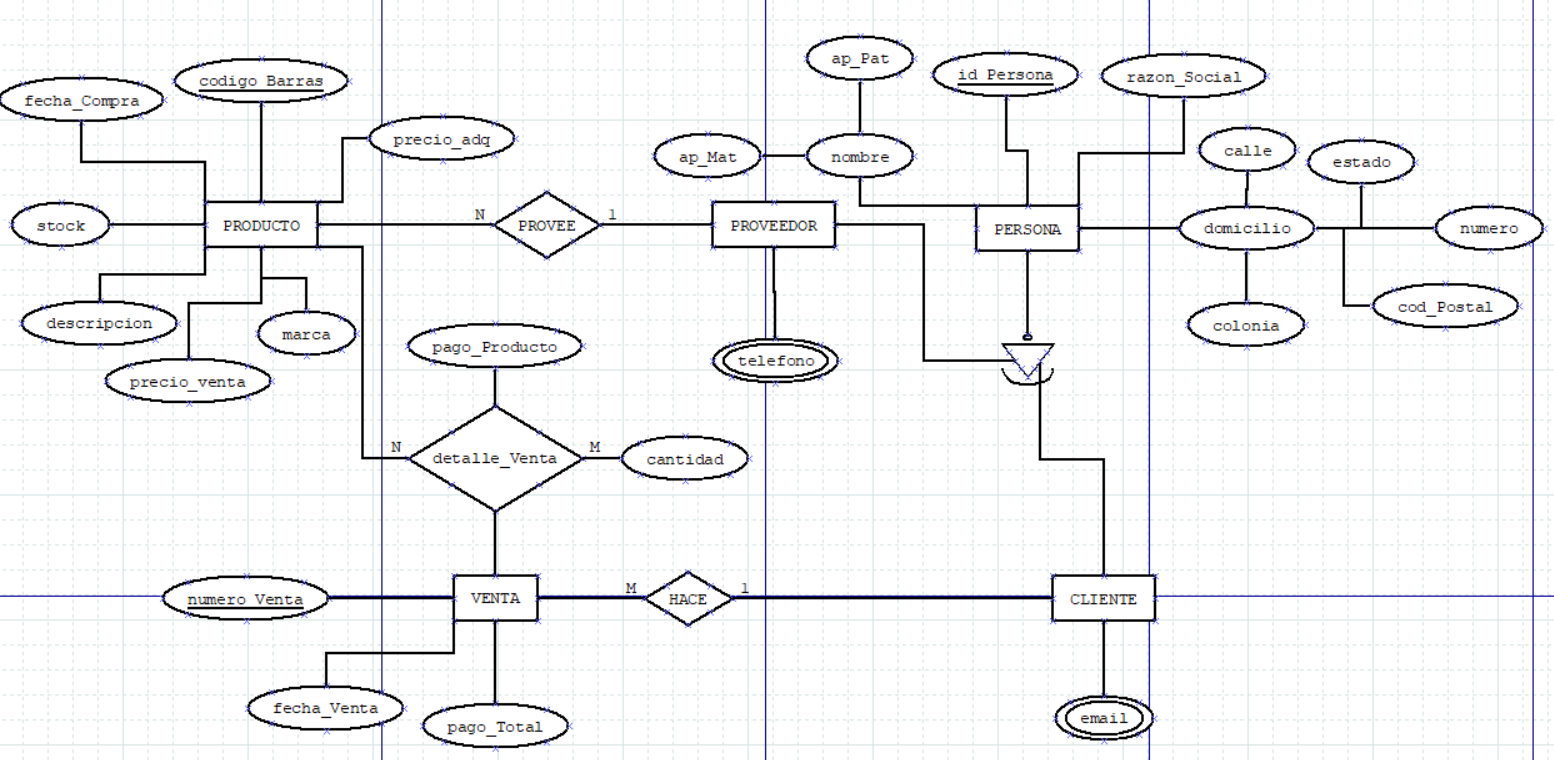
\includegraphics[width=\textwidth]{fig1}
\end{figure}

The next is the logic design, for this we map the entity-relationship model into the relational model but first we have to make the intermediate representation\\

\begin{itemize}
\item First we map the supertype “PERSONA” with its subtypes “PROVEEDOR” and “CLIENTE” by using a method that says: “create a relation for the supertype including all of its attributes, create a new relation for each subtype including the primary key of the supertype and add the attributes of the subtypes”, finally we add a new attribute called “tipo” in order to difference between a supplier and a customer\\

PERSONA \{id\textunderscore Persona (PK), nombre, razón\textunderscore Social, calle, colonia, numero, cod\textunderscore Postal, tipo (CCK), estado\}\\

PROVEEDOR \{(id\textunderscore persona (FK), telefono) (PK)\}\\

CLIENTE \{(id\textunderscore persona (FK), email) (PK)\}\\

\item The next ones will be “PRODUCTO” and “VENTA” these ones are easy since they don’t need a special rule to map, we just need to remember they have one to many relationships so the primary key of the relation with the cardinality one spreads to the relation with the cardinality many

PRODUCTO \{codigo\textunderscore Barras (PK), precio\textunderscore adq, precio\textunderscore venta, marca, descripción, stock, fecha\textunderscore Compra, teléfono (FK), id\textunderscore Persona (FK)\}\\

VENTA \{numero\textunderscore Venta (PK), fecha\textunderscore Venta, pago\textunderscore Total, email (FK), id\textunderscore Persona (FK)\}\\

\item Now we just have to map the many to many relationship for this we create a new relation, spread the primary keys of the entities connected and add the attributes the relationship had.\\

DETALLE\textunderscore VENTA \{(código\textunderscore Barras (FK), numero\textunderscore Venta (FK)) (PK), pago\textunderscore Producto, cantidad\}
\end{itemize}

After deciding some other aspects about the attributes the final result would be:\\

PERSONA \{id\textunderscore Persona (PK), nombre, razón\textunderscore Social, calle, colonia, numero, cod\textunderscore Postal, tipo (CCK), estado\}\\

PROVEEDOR \{(id\textunderscore persona (FK), telefono) (PK)\}\\

CLIENTE \{(id\textunderscore persona (FK), email) (PK), ap\textunderscore pat, ap\textunderscore mat\}\\

PRODUCTO \{codigo\textunderscore Barras (PK), precio\textunderscore adq, precio\textunderscore venta, marca, descripción, stock, fecha\textunderscore Compra, teléfono (FK), id\textunderscore Persona (FK)\}\\

VENTA \{numero\textunderscore Venta (PK), fecha\textunderscore Venta, pago\textunderscore Total, email (FK), id\textunderscore Persona (FK)\}\\

DETALLE\textunderscore VENTA \{(código\textunderscore Barras (FK), numero\textunderscore Venta (FK)) (PK), pago\textunderscore Producto, cantidad\}\\

Creating the relational model having this intermediate representation is as easy as a simple copy-paste we just have to decide the data types of each attribute.\\

\begin{figure}[h]
\caption {Complete relational model}
\centering
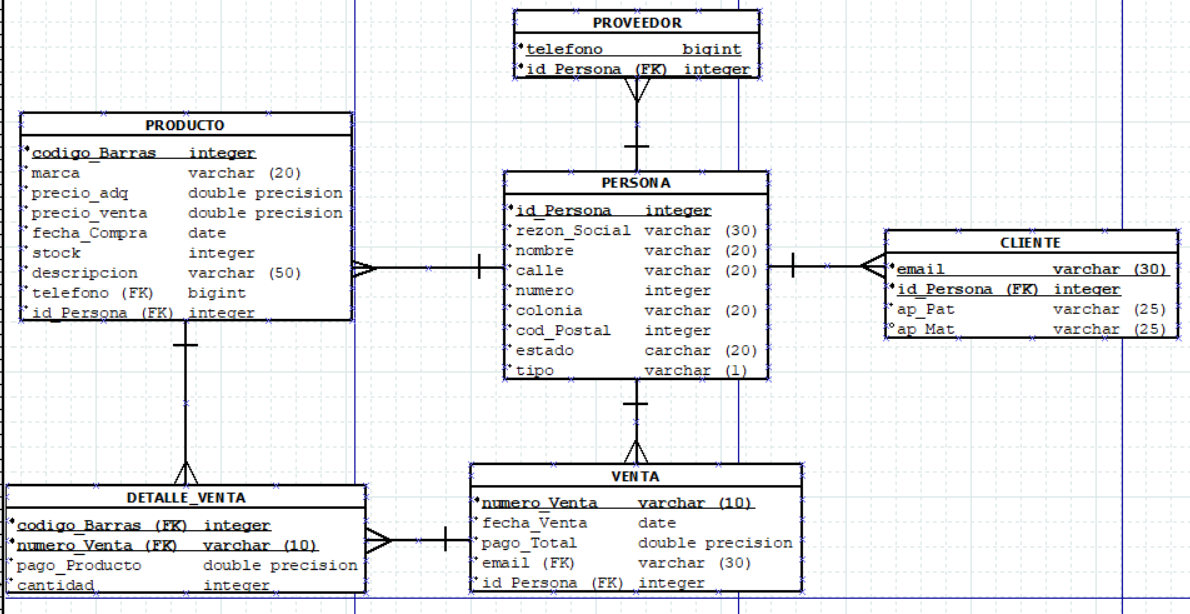
\includegraphics[width=\textwidth]{fig2}
\end{figure}

The final step is the physical design where we implement the database\\

\begin{itemize}
\item PERSONA\\

\begin{lstlisting}
CREATE TABLE public.persona
(
	id_persona integer NOT NULL,
	razon_social character varying(30) COLLATE pg_catalog."default" NOT NULL,
	nombre character varying(20) COLLATE pg_catalog."default" NOT NULL,
	calle character varying(20) COLLATE pg_catalog."default" NOT NULL,
	numero integer NOT NULL,
	colonia character varying(20) COLLATE pg_catalog."default" NOT NULL,
	codigo_postal integer NOT NULL,
	estado character varying(20) COLLATE pg_catalog."default" NOT NULL,
	tipo character varying(1) COLLATE pg_catalog."default" NOT NULL,
	CONSTRAINT persona_pk PRIMARY KEY (id_persona),
	CONSTRAINT persona_tipo_check CHECK (tipo::text = 'c'::text OR 
	tipo::text = 'p'::text)
)
\end{lstlisting}

\item CLIENTE\\

\begin{lstlisting}
CREATE TABLE public.cliente
(
	email character varying(30) COLLATE pg_catalog."default" NOT NULL,
	id_persona integer NOT NULL,
	ap_pat character varying(25) COLLATE pg_catalog."default" NOT NULL,
	ap_mat character varying(25) COLLATE pg_catalog."default",
	CONSTRAINT pk_cliente PRIMARY KEY (email, id_persona),
	CONSTRAINT fk_idpersona FOREIGN KEY (id_persona)
	REFERENCES public.persona (id_persona) MATCH SIMPLE
)
\end{lstlisting}

\item PROVEEDOR\\

\begin{lstlisting}
CREATE TABLE public.proveedor
(
	telefono bigint NOT NULL,
	id_persona integer NOT NULL,
	CONSTRAINT pk_proveedor PRIMARY KEY (telefono, id_persona),
	CONSTRAINT fk_idpersona FOREIGN KEY (id_persona)
	REFERENCES public.persona (id_persona) MATCH SIMPLE
)
\end{lstlisting}

\item PRODUCTO\\

\begin{lstlisting}
CREATE TABLE public.producto
(
	codigo_barras integer NOT NULL,
	marca character varying(20) COLLATE pg_catalog."default" NOT NULL,
	precio_adq double precision NOT NULL,
	precio_venta double precision NOT NULL,
	fecha_compra date NOT NULL,
	stock integer NOT NULL,
	descripcion character varying(50) COLLATE pg_catalog."default" NOT NULL,
	telefono bigint NOT NULL,
	id_persona integer NOT NULL,
	CONSTRAINT producto_pkey PRIMARY KEY (codigo_barras),
	CONSTRAINT fk_proveedor FOREIGN KEY (id_persona, telefono)
	REFERENCES public.proveedor (id_persona, telefono) MATCH SIMPLE,
	CONSTRAINT ck_precioadq CHECK (precio_adq > 0::double precision),
	CONSTRAINT ck_precioventa CHECK (precio_venta > 0::double precision)
)
\end{lstlisting}

\item VENTA\\

\begin{lstlisting}
CREATE TABLE public.venta
(
	numero_venta character varying(10) COLLATE pg_catalog."default" NOT NULL 
	DEFAULT ('VENT-'::text || nextval('secuencia_pkventa'::regclass)),
	fecha_venta date NOT NULL,
	pago_total double precision NOT NULL,
	email character varying(30) COLLATE pg_catalog."default" NOT NULL,
	id_persona integer NOT NULL,
	CONSTRAINT pk_venta PRIMARY KEY (numero_venta),
	CONSTRAINT fk_cliente FOREIGN KEY (email, id_persona)
	REFERENCES public.cliente (email, id_persona) MATCH SIMPLE,
	CONSTRAINT ck_pagototal CHECK (pago_total > 0::double precision)
)
\end{lstlisting}

\item DETALLE\textunderscore VENTA\\

\begin{lstlisting}
CREATE TABLE public.detalle_venta
(
	codigo_barras integer NOT NULL,
	numero_venta character varying(10) COLLATE pg_catalog."default" NOT NULL,
	pago_producto double precision NOT NULL,
	cantidad integer NOT NULL,
	CONSTRAINT pk_detalleventa PRIMARY KEY (codigo_barras, numero_venta),
	CONSTRAINT fk_codigobarras FOREIGN KEY (codigo_barras)
	REFERENCES public.producto (codigo_barras) MATCH SIMPLE
	CONSTRAINT fk_numeroventa FOREIGN KEY (numero_venta)
	REFERENCES public.venta (numero_venta) MATCH SIMPLE
	CONSTRAINT ck_pago CHECK (pago_producto > 0::double precision)
)
\end{lstlisting}
\end{itemize}

\section{Implementation:}

The next section will explain the solution taken to solve each point of the requirements.\\

\begin{itemize}
\item When a barcode of a product is received, return the utility\\

When a bar code is entered, the function searches for the bar code in the table and automatically calculates the profit by subtracting the purchase price from the sale price.\\

\begin{lstlisting}
CREATE FUNCTION utilidad(cod_bar INT)
RETURNS double precision
AS $$
BEGIN
	RETURN precio_venta - precio_adq FROM producto WHERE 
	codigo_barras = cod_bar;
END;
$$ LANGUAGE plpgsql;
\end{lstlisting}

\item Each time a sell is made, the stock must decrease by the selling cuantity. If the value is zero the transaction is aborted. If there is less of three, send a message\\

To fulfill this requirement a function called “actualiza\textunderscore stock” was created\\

First, if the quantity to be reduced from the stock is greater than the stock, a message is sent that says Not enough stock \\

If there are enough stocks then the table is updated and if after updating the table there are less than 3 stocks then a message is sent \\

\begin{lstlisting}
CREATE FUNCTION public.actualiza_stock()
RETURNS trigger
AS $BODY$
BEGIN
	IF (select stock < new.cantidad from producto where 
	codigo_Barras = new.codigo_Barras) 
	THEN 
		RAISE EXCEPTION 'No hay existencias suficientes';
	ELSEIF(select stock >= new.cantidad from producto 
	where codigo_Barras = new.codigo_Barras)
	THEN
		UPDATE PRODUCTO
		SET stock = stock - new.cantidad 
		where codigo_Barras = new.codigo_Barras;
		if (select stock < 3 from producto where 
		codigo_Barras = new.codigo_Barras)
		THEN
			RAISE NOTICE 'Quedan menos de 3 existencias en stock';
		end if;
		return new;
	END IF;
END;
$BODY$;
\end{lstlisting}

\item Given a date or a start date and end date, return the total amount sold of that date/period\\

In this function, all the payments received that are within the entered period are added \\

\begin{lstlisting}
CREATE OR REPLACE FUNCTION public.total_vendido(
	fecini date,
	fecfin date)
	RETURNS double precision
	LANGUAGE 'plpgsql'
	AS $BODY$
BEGIN
	RETURN (SELECT SUM(pago_total) FROM venta WHERE fecha_venta 
	BETWEEN fecini AND fecfin);
END;
$BODY$;
\end{lstlisting}

\item Allow obtaining the name of those products of which there are less than three in stock\\

\begin{lstlisting}
CREATE OR REPLACE FUNCTION public.poco_stock( )
	RETURNS TABLE(descripcion character varying)
	LANGUAGE 'plpgsql'
AS $BODY$
BEGIN
	RETURN QUERY
		SELECT pd.descripcion FROM producto pd WHERE stock < 3;
END;
$BODY$;
\end{lstlisting}

\item Automatically generate a view that contains the necessary information to resemble an invoice\\

A view called “factura” was created where we pick the necessary information from different tables\\

\begin{lstlisting}
CREATE OR REPLACE VIEW public.factura
	AS
	SELECT dv.numero_venta,
		dv.codigo_barras,
		p.descripcion,
		dv.cantidad,
		dv.pago_producto,
		v.pago_total,
		v.fecha_venta,
		v.id_persona,
		per.nombre,
		v.email
		FROM detalle_venta dv
		JOIN venta v ON dv.numero_venta::text = v.numero_venta::text
		JOIN producto p ON dv.codigo_barras = p.codigo_barras
		JOIN persona per ON per.id_persona = v.id_persona;
\end{lstlisting}

\item Create at least, one index of the type that is preferred and where it is preferred. Justify the reason for the choice in both aspects.\\

An index was created in the person table on the name, this in case the data of a person is required and you have to search by the name then the index can speed up the process \\

The index is of hash type because the search would be for equality \\

\begin{lstlisting}
CREATE INDEX idx_name ON persona USING hash;
\end{lstlisting}
\end{itemize}

\section{Presentation:}

The first screen that appears when entering the system is the login screen.\\

\begin{figure}[h]
\caption {Login screen}
\centering
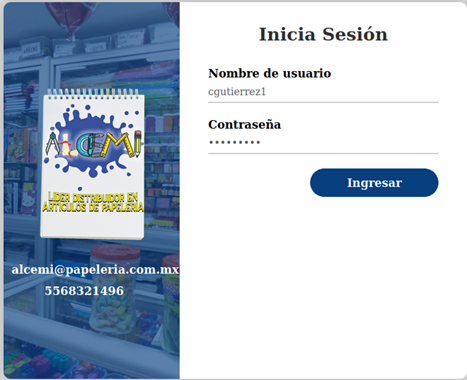
\includegraphics[scale=1]{fig3}
\end{figure}

On this screen we must enter the username and password corresponding to each user, these are provided by the system administrator.\\

\pagebreak

\begin{center}
MAIN MENU
\end{center}
\begin{figure}[ht]
\begin{minipage}[t]{0.5\linewidth}
\caption {Main menu}
\centering
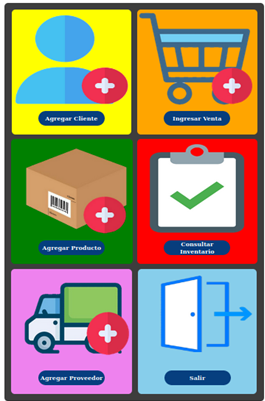
\includegraphics[scale=1]{fig4}
\end{minipage}
\begin{minipage}[t]{0.5\linewidth}
\bigskip
\bigskip
\bigskip
\bigskip
\bigskip
\bigskip
\bigskip
\bigskip
After having correctly entered the data we can access the main menu, where we can register new sales, customers, suppliers and products. In this menu we can also consult the inventory of the products we have, and exit the current session.
\end{minipage}
\end{figure}

\pagebreak

\begin{center}
CLIENT
\end{center}
\begin{figure}[ht]
\begin{minipage}[t]{0.5\linewidth}
\bigskip
\bigskip
\bigskip
\bigskip
\bigskip
\bigskip

The first module allows us to add a client, within this module we must enter the data of the new client: name, paternal surname, maternal surname, company name in case of having one, first email, second email, street, number, colony, code postcard and state. In this section some fields are marked as mandatory by this symbol (*) the data that is not mandatory is the maternal last name, the second email and the company name.\\

Since we fill the entire form, we will press the button "register client" and if everything is correct, the form will send a message confirming the registration.\\
\end{minipage}
\begin{minipage}[t]{0.5\linewidth}
\caption {Client}
\centering
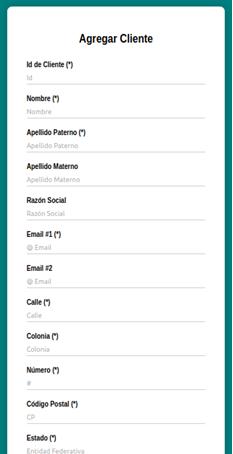
\includegraphics[scale=1]{fig5}
\end{minipage}
\end{figure}

\pagebreak

\begin{center}
SALE
\end{center}
\begin{figure}[ht]
\begin{minipage}[t]{0.5\linewidth}
\caption {Sale}
\centering
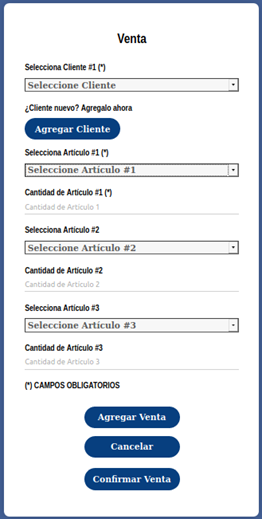
\includegraphics[scale=1]{fig6}
\end{minipage}
\begin{minipage}[t]{0.5\linewidth}
The next module, possibly the most important of all, allows us to add sales.\\

Within this module we must select the client to whom the products will be sold, in case we do not have it registered we have a button in which we can add a new client.\\

After selecting the client, we must select the items to sell, in this part we have a drop-down menu that shows all the products available to sell and just below we must enter the quantity to be sold.\\

We have the possibility of adding 3 different products for each sale.\\

In this module there are more restrictions; If you want to sell a larger quantity than what we have in stock, the system throws an error message and the sale cannot be made. If an incorrect value is entered in the quantity of the product, we will receive an error message indicating that we must enter the correct data.\\

Since we have all the form filled out correctly we can select 3 options: Add sale, cancel or confirm sale, in order to make the sale we must first select add sale and a view of the products we have added will be displayed and what is the price that we will receive for each product and the total payment for the sale.\\

If you want to cancel the sale, we will select the Cancel button.
\end{minipage}
\end{figure}

\pagebreak

\begin{center}
PRODUCT
\end{center}
\begin{figure}[ht]
\begin{minipage}[t]{0.5\linewidth}
\bigskip
\bigskip
\bigskip
\bigskip
The third module is "add product", where we can add new products to our inventory. In this section we must enter the barcode belonging to the product, the description of the product where we can put the name of the product and some extra specification that is needed, the brand of the product, the price at which it was purchased from the supplier, the price at which the customer will be sold, how many pieces we add to the stock and select the supplier who sold us the product, in case a new supplier sells the product, we can select the "Add supplier" button to enter the data of a new provider.\\

Once we have correctly filled out the form we select the "Register Product" button where the registration will be confirmed.\\
\end{minipage}
\begin{minipage}[t]{0.5\linewidth}
\caption {Product}
\centering
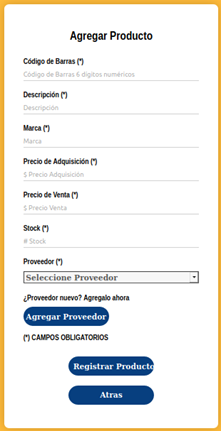
\includegraphics[scale=1]{fig7}
\end{minipage}
\end{figure}

\pagebreak

\begin{center}
CHECK INVENTORY
\end{center}

The next module is "Consult inventory", where there are not many options here since when entering it only shows the data of the products that we have in stock.\\

\begin{figure}[h]
\caption {Check inventory}
\centering
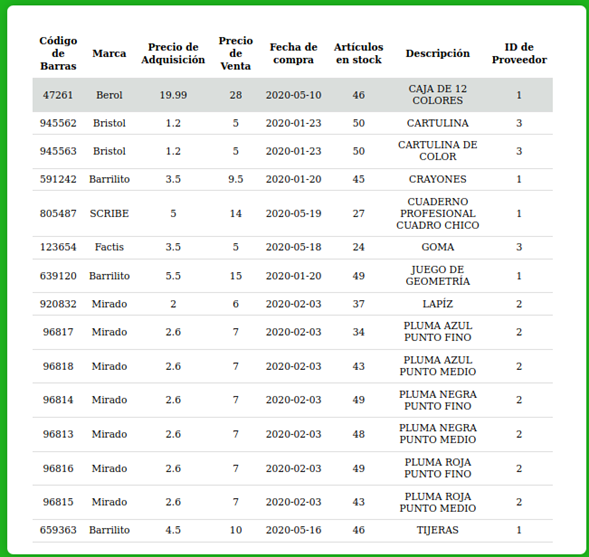
\includegraphics[width=\textwidth]{fig8}
\end{figure}

\pagebreak

\begin{center}
SUPPLIER
\end{center}
\begin{figure}[ht]
\begin{minipage}[t]{0.5\linewidth}
\caption {Supplier}
\centering
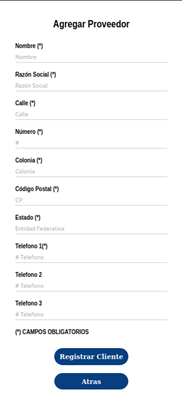
\includegraphics[scale=1]{fig9}
\end{minipage}
\begin{minipage}[t]{0.5\linewidth}
\bigskip
\bigskip
\bigskip
\bigskip
\bigskip
\bigskip
The fifth module allows us to add a new provider, in this form we must enter the data corresponding to the new provider; name, business name, address and 3 contact phone numbers where we must enter at least one phone number.\\

To register the supplier, select the button to register the client and we will receive a message that you have successfully registered.
\end{minipage}
\end{figure}

\pagebreak

\begin{center}
App
\end{center}
Since nowadays everybody use their smartphones to do everything, we decided to also develop an app. This app works in the same way the web page does, having the same menus.\\

\begin{figure}[h]
\begin{minipage}[t]{0.5\linewidth}
\caption {App icon}
\centering

\includegraphics[scale=0.16]{fig10}
\end{minipage}
\begin{minipage}[t]{0.5\linewidth}
\caption {App login}
\centering
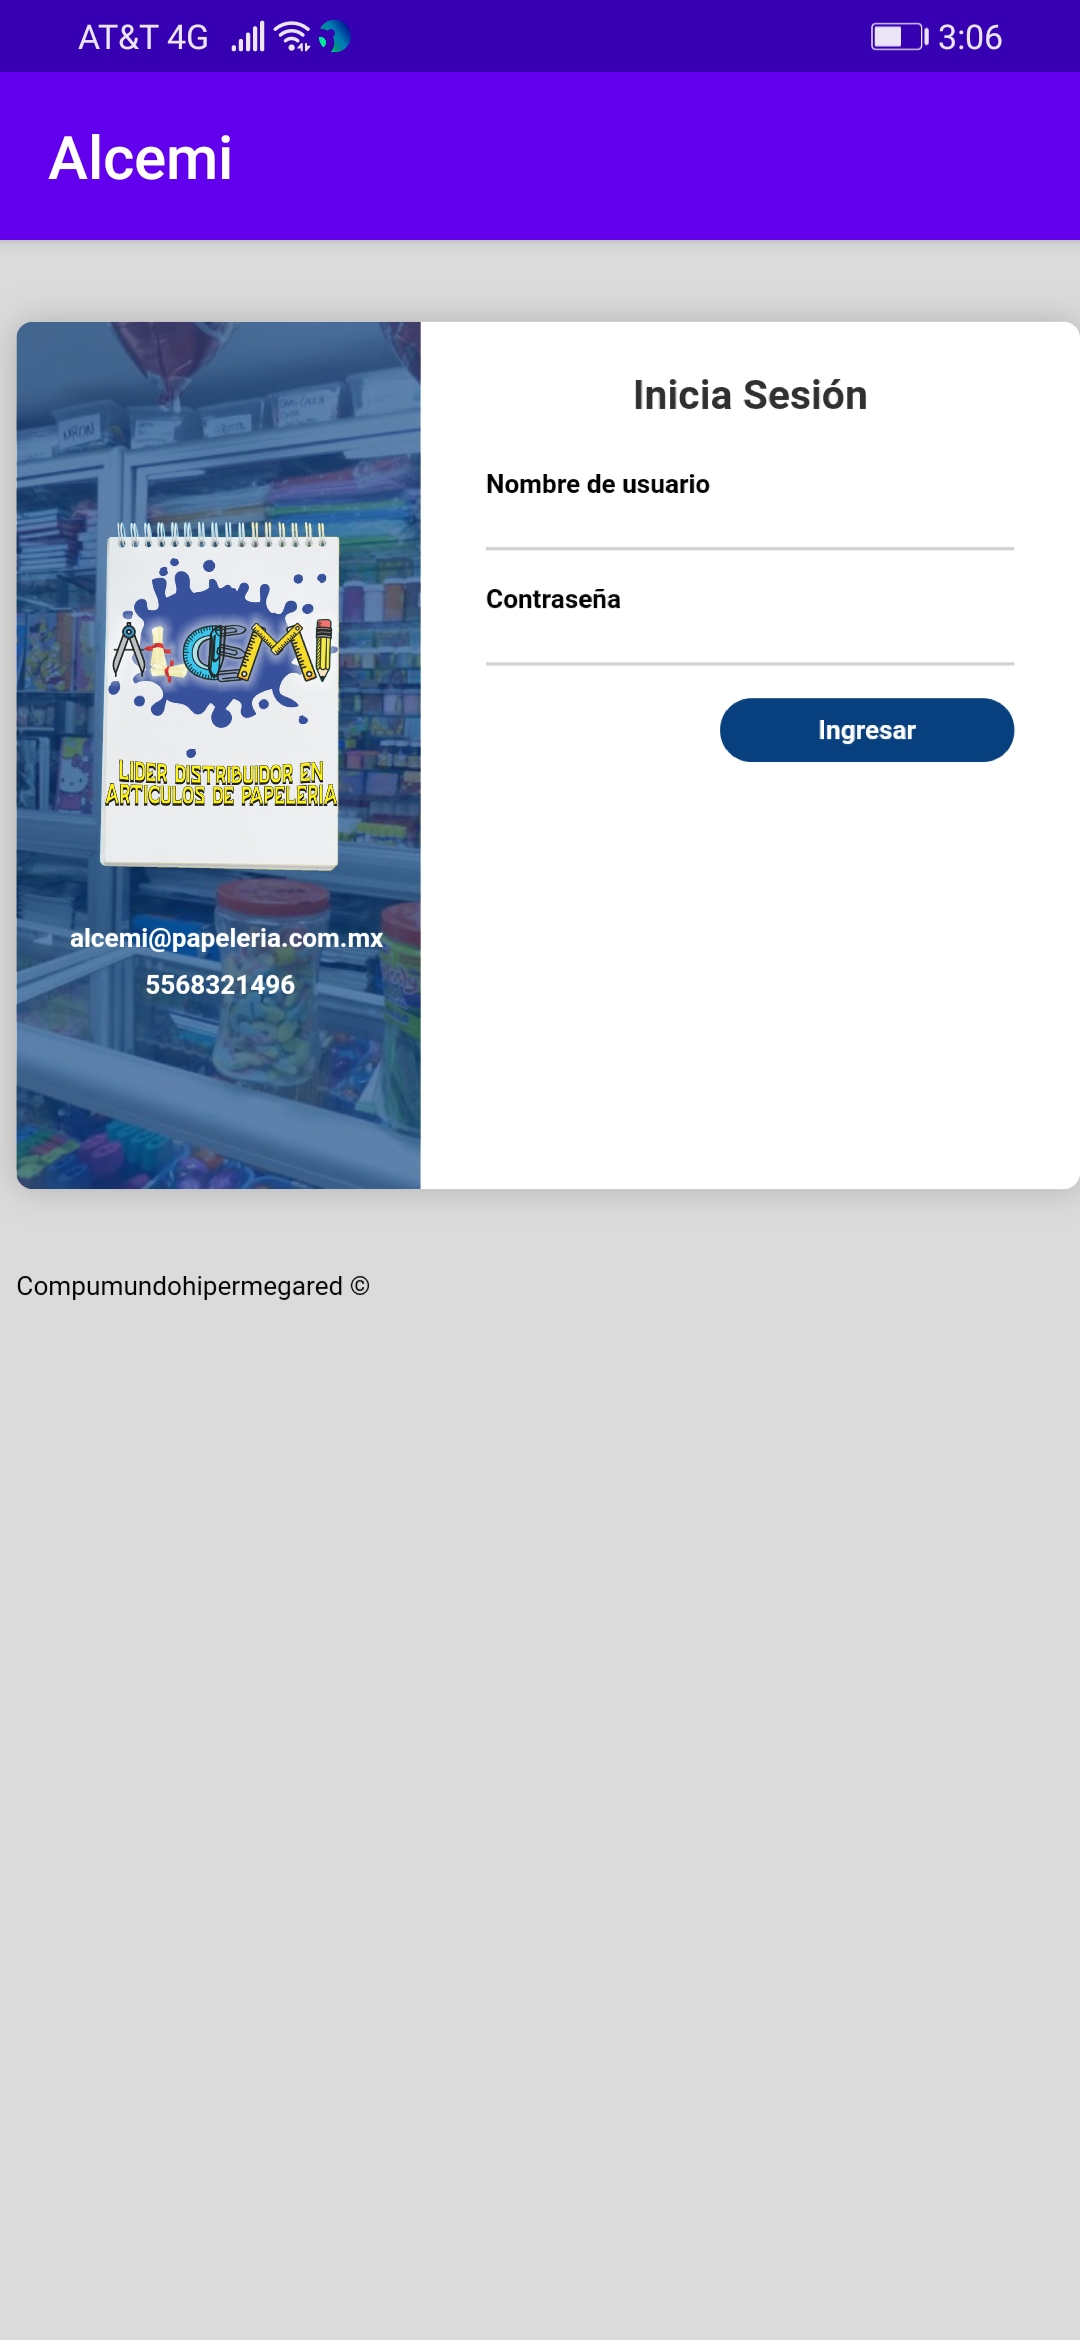
\includegraphics[scale=0.16]{fig11}
\end{minipage}
\end{figure}

\pagebreak

\begin{figure}[h]
\begin{minipage}[t]{0.5\linewidth}
\caption {Main menu}
\centering
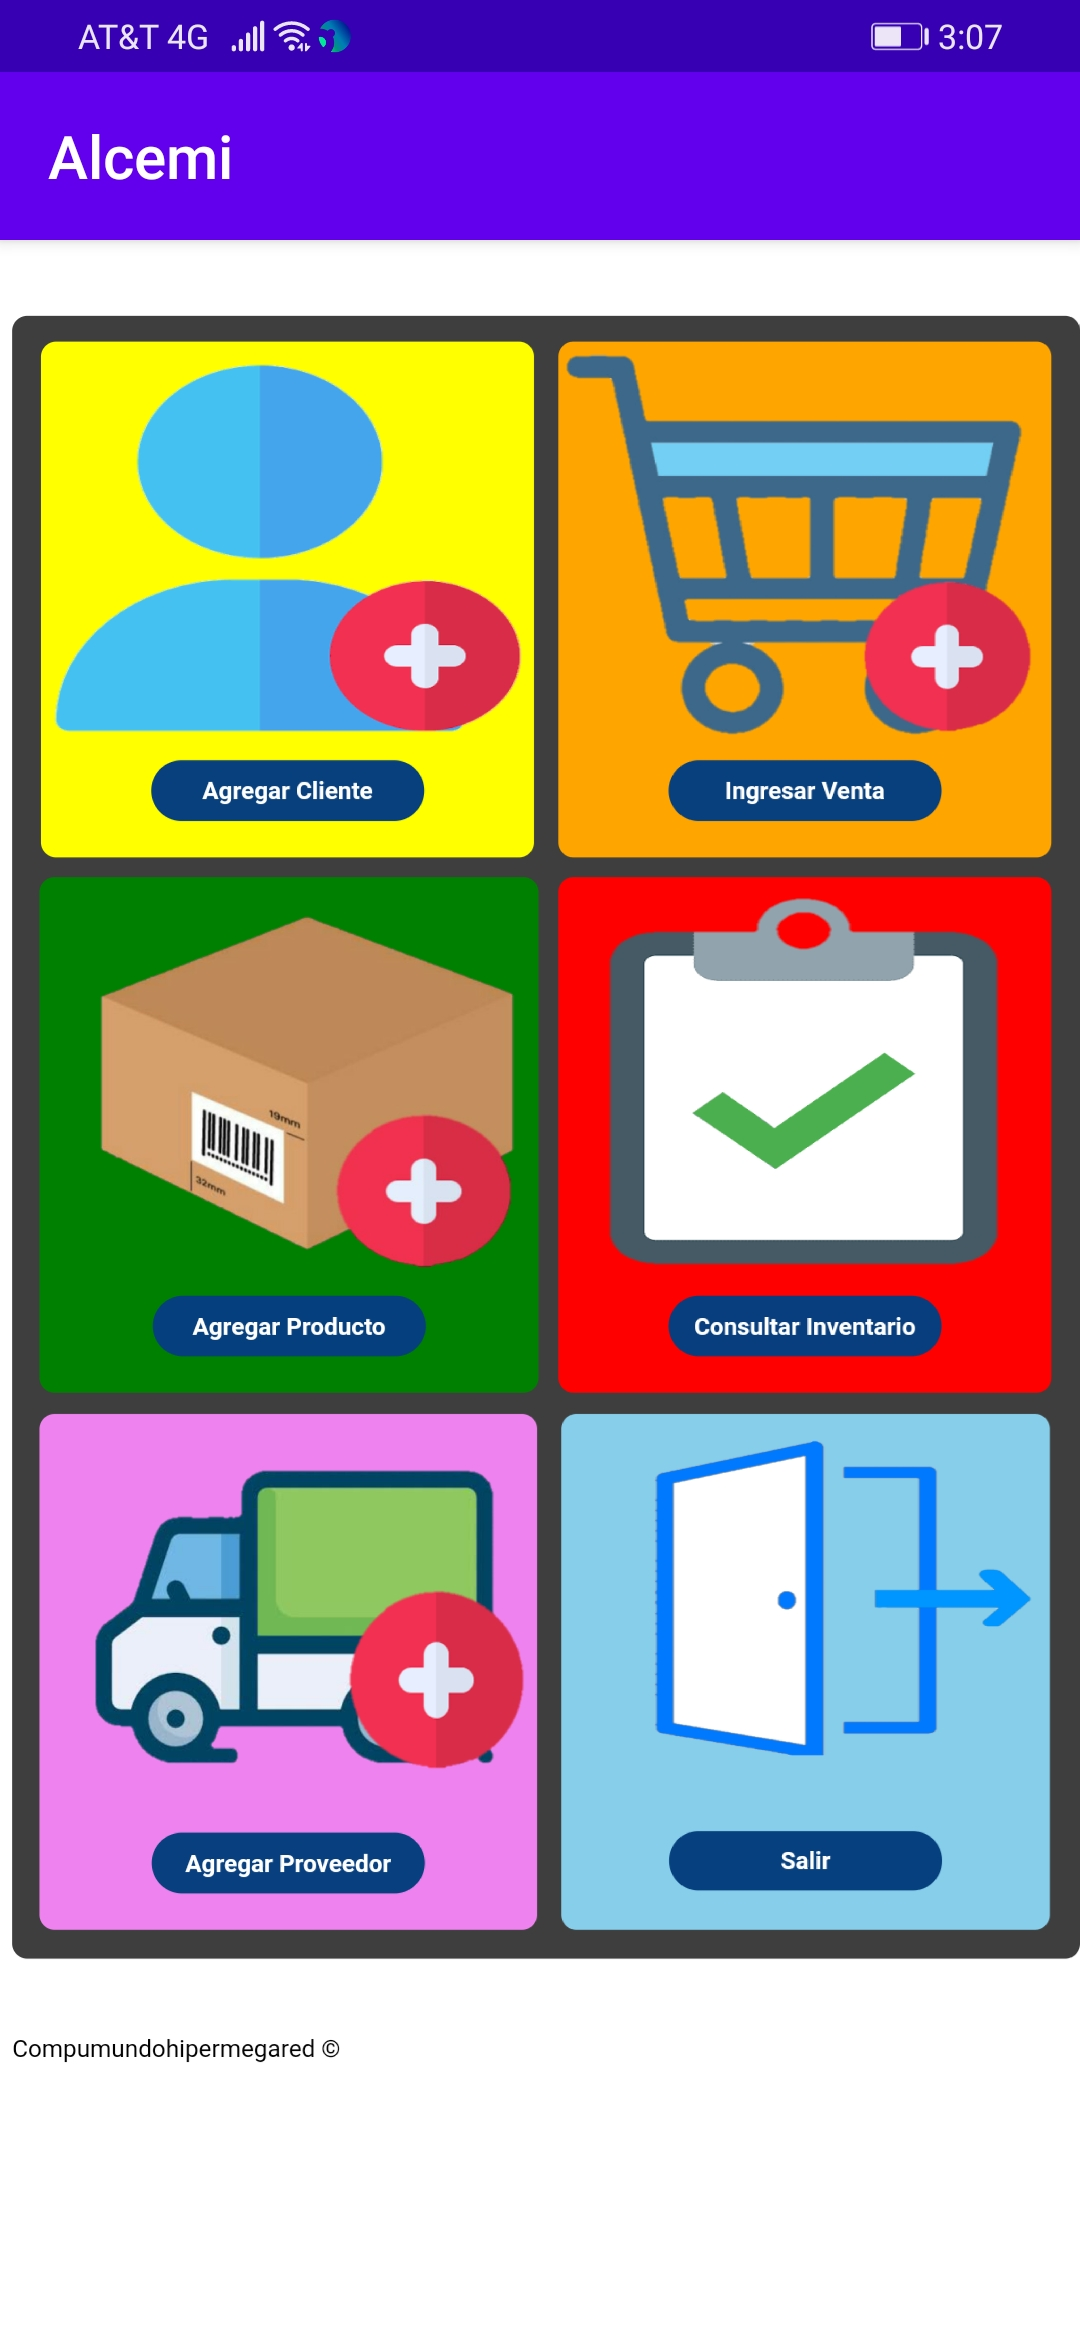
\includegraphics[scale=0.16]{fig12}
\end{minipage}
\begin{minipage}[t]{0.5\linewidth}
\caption {Making a sale}
\centering
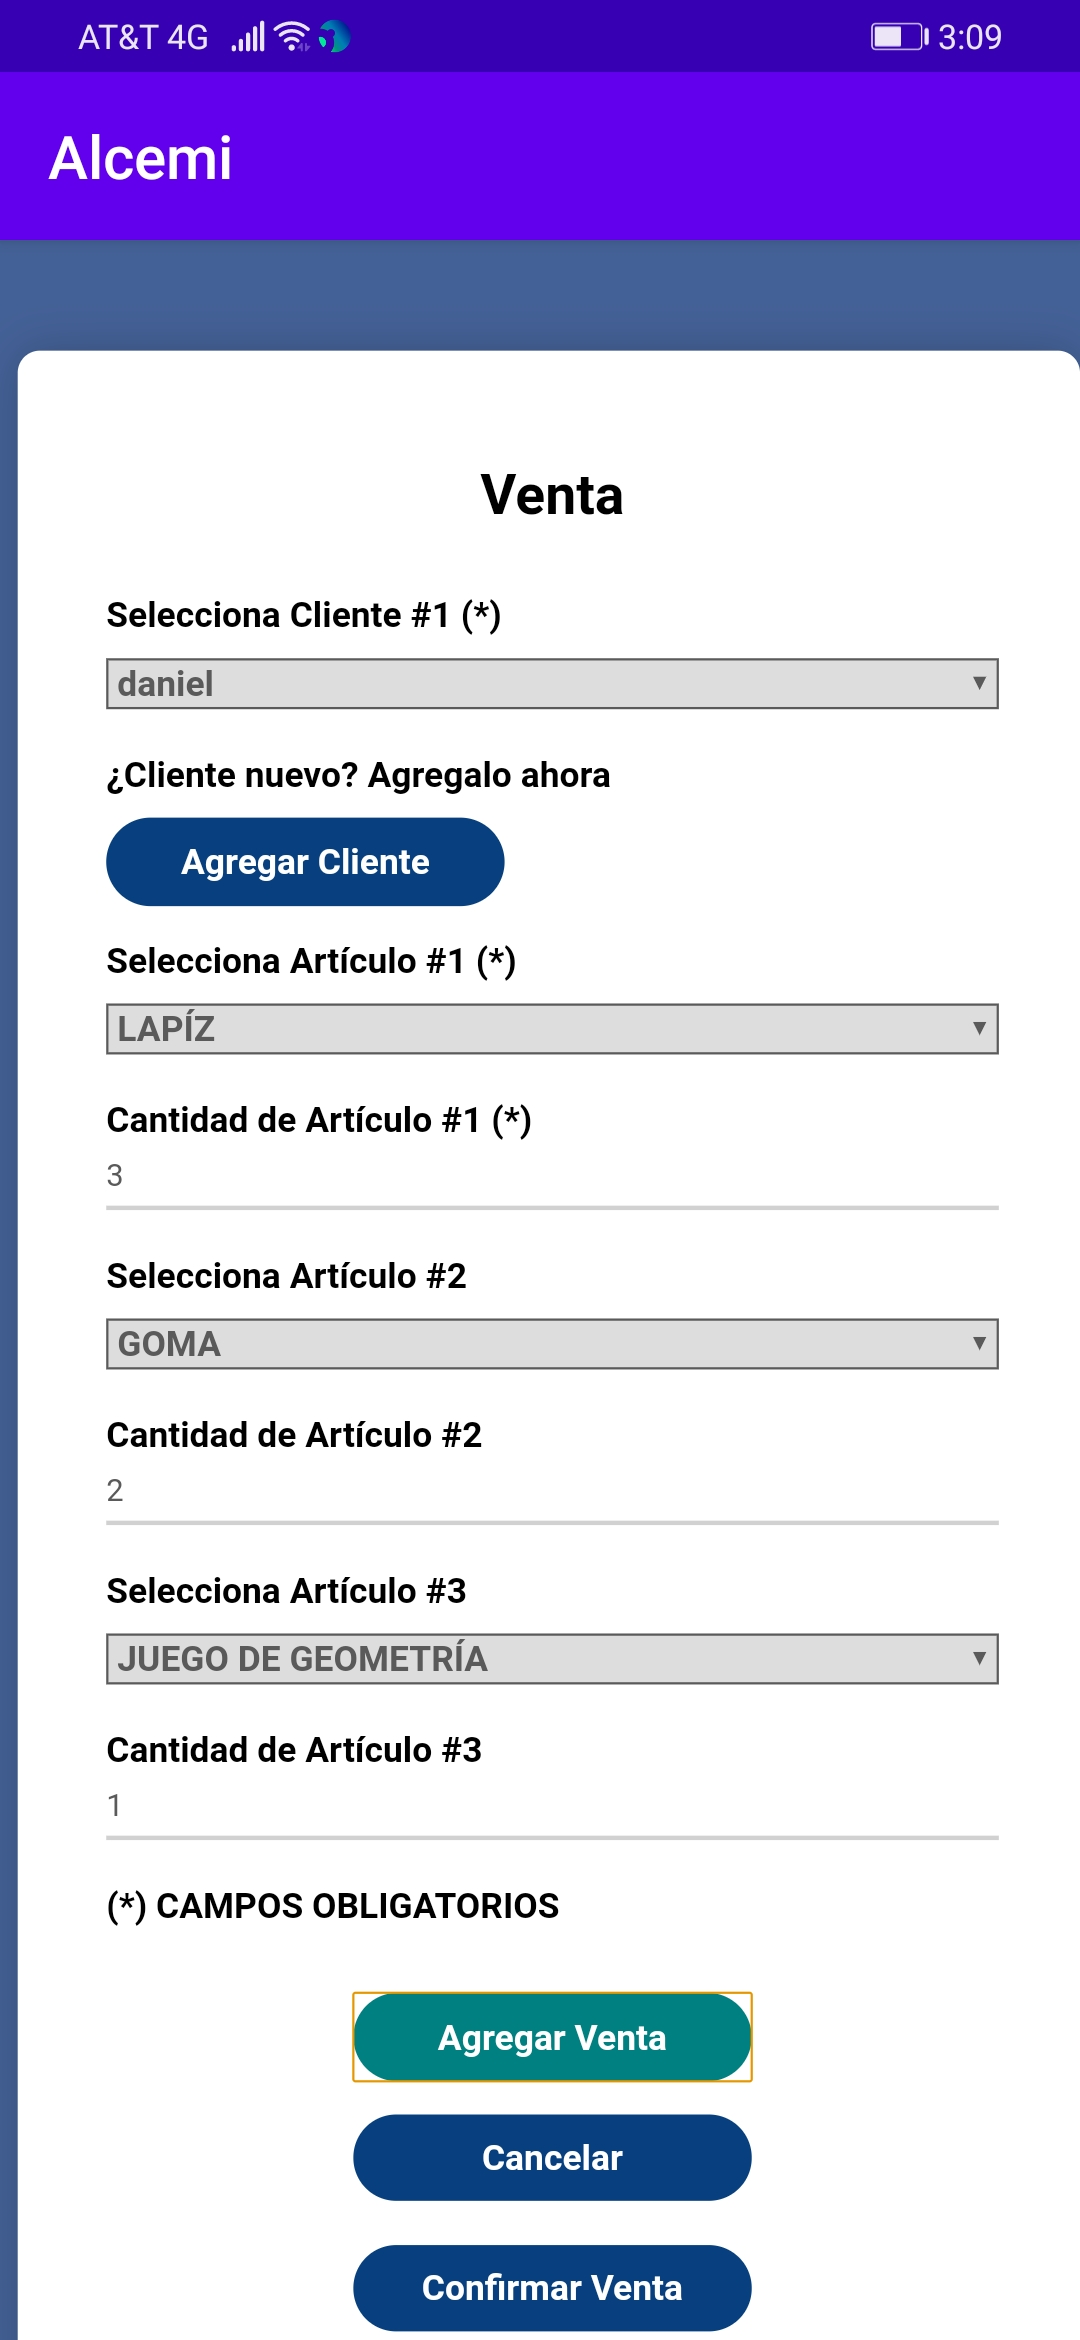
\includegraphics[scale=0.16]{fig13}
\end{minipage}
\end{figure}

\pagebreak

\begin{figure}[h]
\caption {Making a sale}
\centering
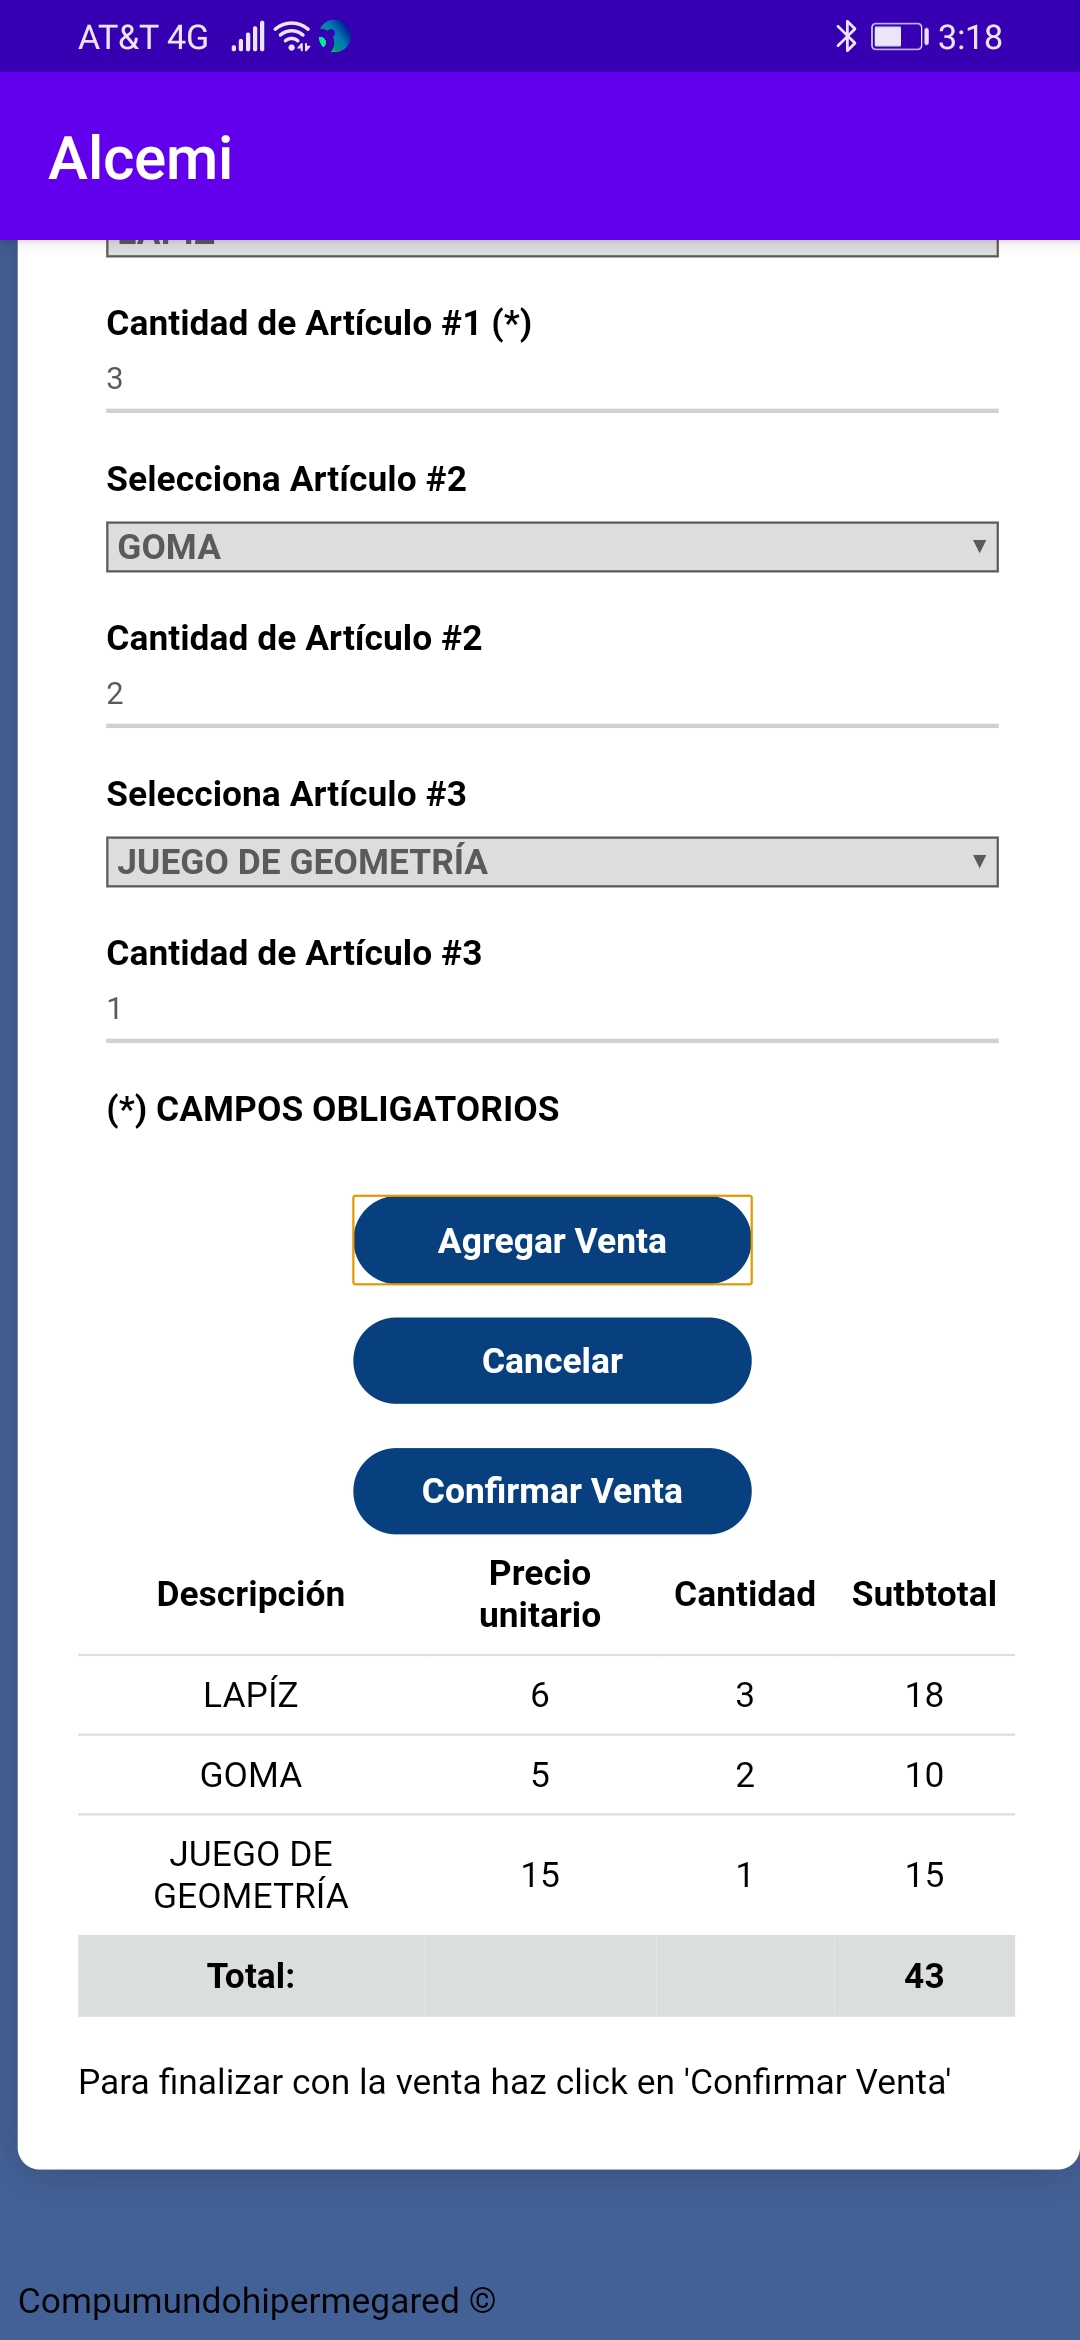
\includegraphics[scale=0.16]{fig14}
\end{figure}

\pagebreak

\section{Conclusions}
César Gutierrez: This project was very useful not only to put into practice everything learned in the course, but it also made us learn many new things, such as those directly related to the creation of the app, for example, and even in the creation of this document.\\

Miguel Guzmán: The realization of this project was very good for the knowledge acquired, since not only what we learned in the course was used, since as the project progressed more opportunities to do new things arose that no one in the team had used before. , such as the management and connection between the servers. At the end of the project we realize that we not only learned databases but also to create a possibly profitable and functional system.\\

Nava Escobar Jose Alfredo: Based on what has been done in this project, I can assure you that participating in it was very enriching, since I was able to put into practice the knowledge acquired throughout the database theorist course in addition to what we as a team learned throughout From the development of our project, teamwork was essential for the realization of this project, I believe that collaboration was the main characteristic of this work team. I am satisfied with the final result since we were able to create and manage a database and likewise create a complete system.\\

\title{Proyecto final (Version en español)}
\author{Compumundohipermegared}
\maketitle

\setcounter{section}{0}
\section{Introduccion}
Este documento describirá el proceso utilizado por nuestro equipo para cumplir con los requisitos del proyecto final. Comenzando con una breve introducción donde mostraremos el análisis del problema y la solución que proponemos, seguido del plan de trabajo que elaboramos y cómo trabajamos cada parte del proyecto en función de las habilidades de cada miembro.\\ 

La siguiente parte detallará el desarrollo de la base de datos a partir del diagrama de entidad-relación que va hasta la interfaz web gráfica, explicando cómo funcionan los procedimientos almacenados, los disparadores, etc. y describiendo la modalidad de conexión que elegimos.\\

La última parte es donde están las conclusiones de cada miembro sobre este proyecto. \\

\section{Plan de trabajo}
El plan de trabajo fue:\\

\begin{itemize}
\item Analizar y entender los requerimientos del cliente para poder realizar un correcto diseño de la base de datos.  
\item Después de comprender los requerimientos comenzamos con la creación del modelo entidad-relación (MER), dónde definimos cuáles serán las principales entidades que contendrá la base de datos y cómo se relacionarán entre sí. 
\item Una vez que creamos el MER pasamos de este modelo a un modelo relacional, dónde podemos especificar mas a fondo cómo será el comportamiento de nuestras relaciones (tablas) y de los datos que se manejarán dónde podremos ver el tipo de datos que manejaremos e incluso algunas reglas de negocio.  
\item Después de revisar nuestro modelo relacional procedemos a la implementación de la base de datos, dónde usaremos el manejador PostgreSQL para desarrollar nuestra base de datos.  
\item Una vez que tenemos la base de datos completa, procedemos a registrar datos para realizar pruebas sobre el comportamiento de la base de datos y corregir problemas que se llegaron a presentar durante la implementación. 
\item Después de tener una base de datos funcionando correcta y establemente se desarrolló el sitió web que funcionará como un punto de venta.  
\item Ya que se levantó el servicio web y el sitio web funciona correctamente se conecta ambos servicios; el servicio web y el servicio de base de datos Postgresql.  
\item Una vez que se conectaron ambos servicios nos enfocamos en realizar pruebas realizando todo tipo de inserciones y casos de uso que pueda presentar cualquier usuario para poder mitigar cualquier posibilidad de que el sistema falle.  
\item Cuándo el equipo haya realizado todas las pruebas necesarias se decidirá dar por finalizado el sistema y concluir el proyecto presentando y entregándolo al usuario.  
\end{itemize}

Las actividades que realizó cada integrante de equipo fueron las siguientes:\\

Análisis del problema y requerimientos del usuario.\- Todo el equipo.\\

Diseño y modelado de la base de datos. \- Todo el equipo.\\

Implementación de la base de datos. \- Todo el equipo.\\

Desarrollo de sitio web. \- Alfredo Nava.\\

Conexión entre servicios y prueba de errores del sistema. \- Miguel Guzmán.\\

Diseño y desarrollo de aplicación web. \- César Gutierrez.\\

Documentación. \- César Gutierrez.\\

\section{Diseño}

De acuerdo con las tres fases del diseño de una base de datos, debemos comenzar por el diseño conceptual\\

Para esto creamos un modelo de relación de entidad donde seleccionamos todas las entidades posibles, luego identificamos sus posibles atributos, después de elegir las entidades necesarias, terminamos con cuatro entidades ("PRODUCTO", "VENTA", "PROVEEDOR" y "CLIENTE") con sus atributos correspondientes, entonces nos dimos cuenta de que dos de esas entidades compartían la mayoría de sus atributos, por lo que creamos un super-tipo para esas dos ("PERSONA"), esta relación será exclusiva porque una persona no puede ser un proveedor y un cliente al mismo tiempo; y total porque la persona DEBE ser un proveedor o un cliente\\

El siguiente paso fue decidir cómo se relacionaría cada entidad entre sí, para hacer esto, prestamos especial atención a los requisitos y consideraciones dados, por lo que creamos tres relaciones (“provee”, “detalle\textunderscore Venta” y “hace”) una de ellas. siendo muchos para muchos y los otros dos siendo uno para muchos.\\

\pagebreak

\setcounter{figure}{0}
\begin{figure}[h]
\caption {Modelo entidad relacion completo}
\centering
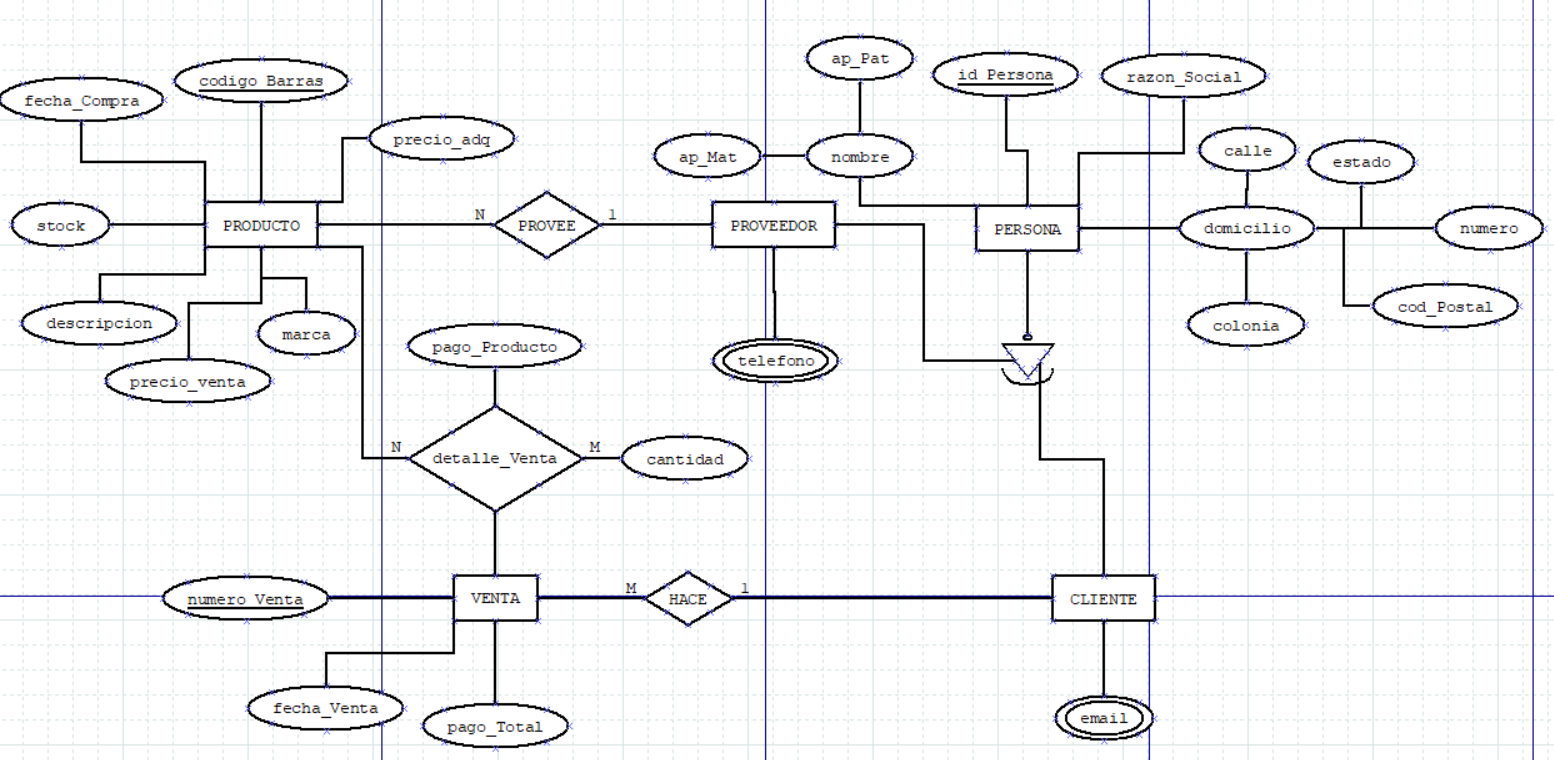
\includegraphics[width=\textwidth]{fig1}
\end{figure}

El siguiente es el diseño lógico, para esto mapeamos el modelo de entidad-relación en el modelo relacional, pero primero tenemos que hacer la representación intermedia. \\

\begin{itemize}
\item Primero mapeamos el super-tipo "PERSONA" con sus subtipos "PROVEEDOR" y "CLIENTE" usando un método que dice: "crear una relación para el super-tipo que incluya todos sus atributos, en la nueva relación agregue los atributos de los subtipos", finalmente agregamos un nuevo atributo llamado "tipo" para diferenciar entre un proveedor y un cliente\\

PERSONA \{id\textunderscore Persona (PK), nombre, razón\textunderscore Social, calle, colonia, numero, cod\textunderscore Postal, tipo (CCK), telefono, email\} \\

PROVEEDOR \{(id\textunderscore persona (FK), telefono) (PK)\} \\

CLIENTE \{(id\textunderscore persona (FK), email) (PK)\} \\

\item Los siguientes serán "PRODUCTO" y "VENTA", estos son fáciles ya que no necesitan una regla especial para mapear, solo necesitamos recordar que tienen una o muchas relaciones, por lo que la clave principal de la relación con la cardinalidad es se extiende a la relación con la cardinalidad muchos \\

PRODUCTO \{codigo\textunderscore Barras (PK), precio\textunderscore adq, precio\textunderscore venta, marca, descripción, stock, fecha\textunderscore Compra, teléfono (FK), id\textunderscore Persona (FK)\} \\

VENTA \{numero\textunderscore Venta (PK), fecha\textunderscore Venta, pago\textunderscore Total, email (FK), id\textunderscore Persona (FK)\} \\

\item Ahora solo tenemos que mapear la relación de muchos a muchos para esto, creamos una nueva relación, separamos las claves primarias de las entidades conectadas y agregamos los atributos que tenía la relación. \\
\end{itemize}

DETALLE\textunderscore VENTA \{(código\textunderscore Barras (FK), numero\textunderscore Venta (FK)) (PK), pago\textunderscore Producto, cantidad\} \\

Después de decidir algunos otros aspectos sobre los atributos, el resultado final sería: \\

PERSONA \{id\textunderscore Persona (PK), nombre, razón\textunderscore Social, calle, colonia, numero, cod\textunderscore Postal, tipo (CCK), estado\}\\ 

PROVEEDOR \{(id\textunderscore persona (FK), telefono) (PK)\} \\

CLIENTE \{(id\textunderscore persona (FK), email) (PK), ap\textunderscore pat, ap\textunderscore mat\} \\

PRODUCTO \{codigo\textunderscore Barras (PK), precio\textunderscore adq, precio\textunderscore venta, marca, descripción, stock, fecha\textunderscore Compra, teléfono (FK), id\textunderscore Persona (FK)\} \\

VENTA \{numero\textunderscore Venta (PK), fecha\textunderscore Venta, pago\textunderscore Total, email (FK), id\textunderscore Persona (FK)\} \\

DETALLE\textunderscore VENTA \{(código\textunderscore Barras (FK), numero\textunderscore Venta (FK)) (PK), pago\textunderscore Producto, cantidad\}\\

Crear el modelo relacional que tiene esta representación intermedia es tan fácil como copiar y pegar, solo tenemos que decidir los tipos de datos de cada atributo. \\

\begin{figure}[h]
\caption {Modelo relacional completo}
\centering
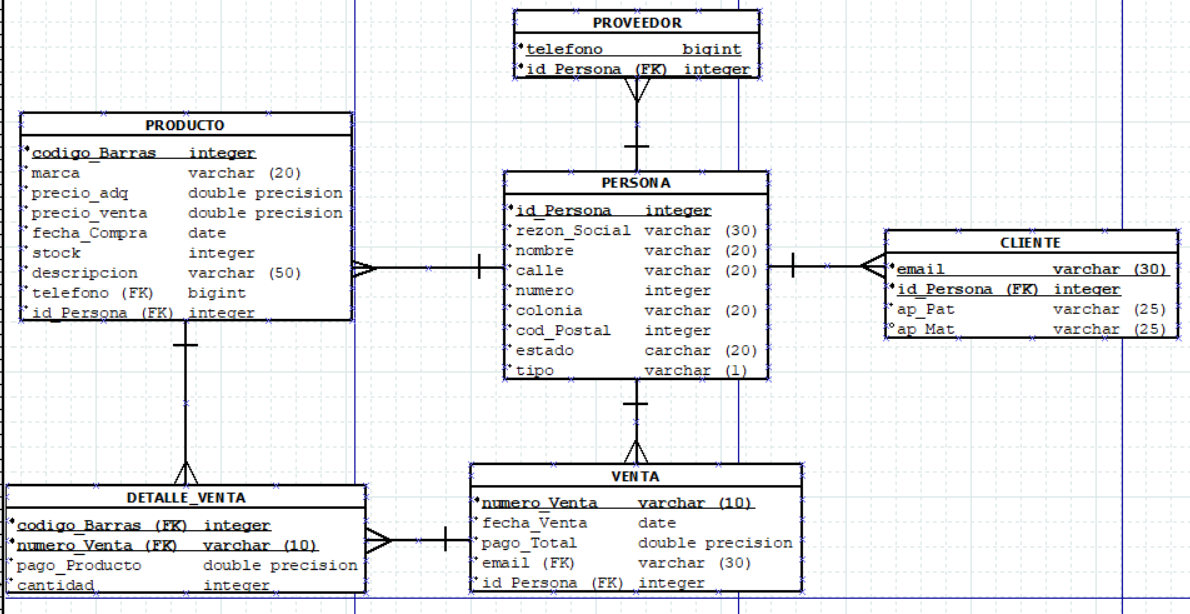
\includegraphics[width=\textwidth]{fig2}
\end{figure}

El paso final es el diseño físico donde implementamos la base de datos. \\

\begin{itemize}
\item PERSONA\\

\begin{lstlisting}
CREATE TABLE public.persona 
( 
	id_persona integer NOT NULL, 
	razon_social character varying(30) COLLATE pg_catalog."default" NOT NULL, 
	nombre character varying(20) COLLATE pg_catalog."default" NOT NULL, 
	calle character varying(20) COLLATE pg_catalog."default" NOT NULL, 
	numero integer NOT NULL, 
	colonia character varying(20) COLLATE pg_catalog."default" NOT NULL, 
	codigo_postal integer NOT NULL, 
	estado character varying(20) COLLATE pg_catalog."default" NOT NULL, 
	tipo character varying(1) COLLATE pg_catalog."default" NOT NULL, 
	CONSTRAINT persona_pk PRIMARY KEY (id_persona), 
	CONSTRAINT persona_tipo_check CHECK (tipo::text = 'c'::text OR
	tipo::text = 'p'::text) 
)
\end{lstlisting}

\item CLIENTE \\

\begin{lstlisting}
CREATE TABLE public.cliente 
( 
	email character varying(30) COLLATE pg_catalog."default" NOT NULL, 
	id_persona integer NOT NULL, 
	ap_pat character varying(25) COLLATE pg_catalog."default" NOT NULL, 
	ap_mat character varying(25) COLLATE pg_catalog."default", 
	CONSTRAINT pk_cliente PRIMARY KEY (email, id_persona), 
	CONSTRAINT fk_idpersona FOREIGN KEY (id_persona) 
	REFERENCES public.persona (id_persona) MATCH SIMPLE 
) 
\end{lstlisting}
 
\item PROVEEDOR \\

\begin{lstlisting}
CREATE TABLE public.proveedor 
( 
	telefono bigint NOT NULL, 
	id_persona integer NOT NULL, 
	CONSTRAINT pk_proveedor PRIMARY KEY (telefono, id_persona), 
	CONSTRAINT fk_idpersona FOREIGN KEY (id_persona) 
	REFERENCES public.persona (id_persona) MATCH SIMPLE 
) 
\end{lstlisting}

\item PRODUCTO \\

\begin{lstlisting}
CREATE TABLE public.producto
(
	codigo_barras integer NOT NULL,
	marca character varying(20) COLLATE pg_catalog."default" NOT NULL,
	precio_adq double precision NOT NULL,
	precio_venta double precision NOT NULL,
	fecha_compra date NOT NULL,
	stock integer NOT NULL,
	descripcion character varying(50) COLLATE pg_catalog."default" NOT NULL,
	telefono bigint NOT NULL,
	id_persona integer NOT NULL,
	CONSTRAINT producto_pkey PRIMARY KEY (codigo_barras),
	CONSTRAINT fk_proveedor FOREIGN KEY (id_persona, telefono)
	REFERENCES public.proveedor (id_persona, telefono) MATCH SIMPLE,
	CONSTRAINT ck_precioadq CHECK (precio_adq > 0::double precision),
	CONSTRAINT ck_precioventa CHECK (precio_venta > 0::double precision)
)
\end{lstlisting}

\item VENTA\\

\begin{lstlisting}
CREATE TABLE public.venta
(
	numero_venta character varying(10) COLLATE pg_catalog."default" NOT NULL 
	DEFAULT ('VENT-'::text || nextval('secuencia_pkventa'::regclass)),
	fecha_venta date NOT NULL,
	pago_total double precision NOT NULL,
	email character varying(30) COLLATE pg_catalog."default" NOT NULL,
	id_persona integer NOT NULL,
	CONSTRAINT pk_venta PRIMARY KEY (numero_venta),
	CONSTRAINT fk_cliente FOREIGN KEY (email, id_persona)
	REFERENCES public.cliente (email, id_persona) MATCH SIMPLE,
	CONSTRAINT ck_pagototal CHECK (pago_total > 0::double precision)
)
\end{lstlisting}

\item DETALLE\textunderscore VENTA\\

\begin{lstlisting}
CREATE TABLE public.detalle_venta
(
	codigo_barras integer NOT NULL,
	numero_venta character varying(10) COLLATE pg_catalog."default" NOT NULL,
	pago_producto double precision NOT NULL,
	cantidad integer NOT NULL,
	CONSTRAINT pk_detalleventa PRIMARY KEY (codigo_barras, numero_venta),
	CONSTRAINT fk_codigobarras FOREIGN KEY (codigo_barras)
	REFERENCES public.producto (codigo_barras) MATCH SIMPLE
	CONSTRAINT fk_numeroventa FOREIGN KEY (numero_venta)
	REFERENCES public.venta (numero_venta) MATCH SIMPLE
	CONSTRAINT ck_pago CHECK (pago_producto > 0::double precision)
)
\end{lstlisting}
\end{itemize} 

\section{Implementacion}
La siguiente sección explicará la solución tomada para resolver cada punto de los requisitos.\\

\begin{itemize}
\item Cuando se recibe un código de barras de un producto, devuelva la utilidad \\

Cuando se ingresa un codigo de barras, la funcion busca el codigo de barras en la tabla y calcula automaticamente la utilidad restando al precio de venta el precio de adquisicion\\

\begin{lstlisting}
CREATE FUNCTION utilidad(cod_bar INT)
RETURNS double precision
AS $$
BEGIN
	RETURN precio_venta - precio_adq FROM producto WHERE 
	codigo_barras = cod_bar;
END;
$$ LANGUAGE plpgsql;
\end{lstlisting}

\item Cada vez que se realiza una venta, la acción debe disminuir según la cantidad de ventas. Si el valor es cero, la transacción se cancela. Si hay menos de tres, envíe un mensaje \\

Para cumplir este requisito, se creó una función llamada "actualización\textunderscore stock"\\

Primero si la cantidad que se va a reducir del stock es mayor al stock se envia un mensaje que dice No hay existencias suficientes\\

Si hay existencias suficientes entonces se actualiza la tabla y si despues de actualizar la tabla quedan menos de 3 existencias entonces se envia un mensaje\\

\begin{lstlisting}
CREATE FUNCTION public.actualiza_stock()
RETURNS trigger
AS $BODY$
BEGIN
	IF (select stock < new.cantidad from producto where 
	codigo_Barras = new.codigo_Barras) 
	THEN 
		RAISE EXCEPTION 'No hay existencias suficientes';
	ELSEIF(select stock >= new.cantidad from producto 
	where codigo_Barras = new.codigo_Barras)
	THEN
		UPDATE PRODUCTO
		SET stock = stock - new.cantidad 
		where codigo_Barras = new.codigo_Barras;
		if (select stock < 3 from producto where 
		codigo_Barras = new.codigo_Barras)
		THEN
			RAISE NOTICE 'Quedan menos de 3 existencias en stock';
		end if;
		return new;
	END IF;
END;
$BODY$;
\end{lstlisting}

\item Dada una fecha o una fecha de inicio y finalización, devuelva la cantidad total vendida de esa fecha / período. \\

En esta funcion se suma todos los pagos recibidos que se encuentren dentro del periodo ingresado\\

\begin{lstlisting}
CREATE OR REPLACE FUNCTION public.total_vendido(
	fecini date,
	fecfin date)
	RETURNS double precision
	LANGUAGE 'plpgsql'
	AS $BODY$
BEGIN
	RETURN (SELECT SUM(pago_total) FROM venta WHERE fecha_venta 
	BETWEEN fecini AND fecfin);
END;
$BODY$;
\end{lstlisting}

\item Permitir obtener el nombre de aquellos productos de los cuales hay menos de tres en stock \\

\begin{lstlisting}
CREATE OR REPLACE FUNCTION public.poco_stock( )
	RETURNS TABLE(descripcion character varying)
	LANGUAGE 'plpgsql'
AS $BODY$
BEGIN
	RETURN QUERY
		SELECT pd.descripcion FROM producto pd WHERE stock < 3;
END;
$BODY$;
\end{lstlisting}

\item Genere automáticamente una vista que contenga la información necesaria para parecerse a una factura. \\

Se creó una vista llamada "factura" donde seleccionamos la información necesaria de diferentes tablas \\

\begin{lstlisting}
CREATE OR REPLACE VIEW public.factura
	AS
	SELECT dv.numero_venta,
		dv.codigo_barras,
		p.descripcion,
		dv.cantidad,
		dv.pago_producto,
		v.pago_total,
		v.fecha_venta,
		v.id_persona,
		per.nombre,
		v.email
		FROM detalle_venta dv
		JOIN venta v ON dv.numero_venta::text = v.numero_venta::text
		JOIN producto p ON dv.codigo_barras = p.codigo_barras
		JOIN persona per ON per.id_persona = v.id_persona;
\end{lstlisting}

\item Cree al menos un índice del tipo que se prefiere y donde se prefiere. Justifique la razón de la elección en ambos aspectos. \\

Se creo un indice en la tabla persona sobre el nombre, esto por si se requieren los datos de una persona y hay que buscar por el nombre entonces el indice puede acelerar el proceso\\

El indice es de tipo hash debido a que la busqueda seria por igualdad\\

\begin{lstlisting}
CREATE INDEX idx_name ON persona USING hash;
\end{lstlisting}
\end{itemize}

\section{Presentacion}

La primer pantalla que aparece cuando se entra al sistema es la pantalla de login.\\

\begin{figure}[h]
\caption {Pantalla de login}
\centering
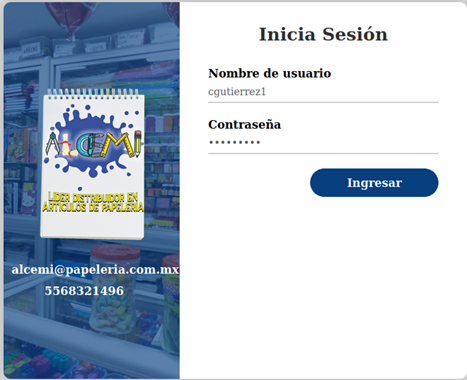
\includegraphics[scale=1]{fig3}
\end{figure}

En esta pantalla debemos ingresar el nombre de usuario y la contraseña correspondientes para cada usuario, estos son provistos por el administrador del sistema.\\

\pagebreak

\begin{center}
MENU PRINCIPAL
\end{center}
\begin{figure}[ht]
\begin{minipage}[t]{0.5\linewidth}
\caption {Menu principal}
\centering
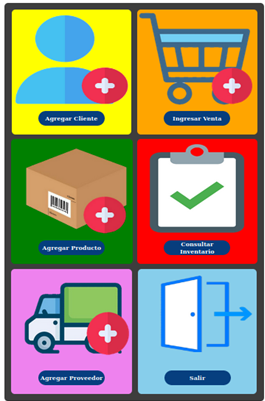
\includegraphics[scale=1]{fig4}
\end{minipage}
\begin{minipage}[t]{0.5\linewidth}
\bigskip
\bigskip
\bigskip
\bigskip
\bigskip
\bigskip
\bigskip
\bigskip
Después de haber ingresado correctamente los datos, podemos acceder al menú principal, donde podemos registrar nuevas ventas, clientes, proveedores y productos. En este menú también podemos consultar el inventario de los productos que tenemos y salir de la sesión actual. 
\end{minipage}
\end{figure}

\pagebreak

\begin{center}
CLIENTE
\end{center}
\begin{figure}[ht]
\begin{minipage}[t]{0.5\linewidth}
\bigskip
\bigskip
\bigskip
\bigskip
\bigskip
\bigskip

El primer módulo nos permite agregar un cliente, dentro de este módulo debemos ingresar los datos del nuevo cliente: nombre, apellido paterno, apellido materno, nombre de la empresa en caso de tener uno, primer correo electrónico, segundo correo electrónico, calle, número, colonia , código postal y estado. En esta sección, algunos campos están marcados como obligatorios con este símbolo (*). Los datos que no son obligatorios son el apellido materno, el segundo correo electrónico y el nombre de la empresa. \\

Como llenamos el formulario completo, presionaremos el botón "registrar cliente" y si todo está correcto, el formulario enviará un mensaje confirmando el registro. \\
\end{minipage}
\begin{minipage}[t]{0.5\linewidth}
\caption {Cliente}
\centering
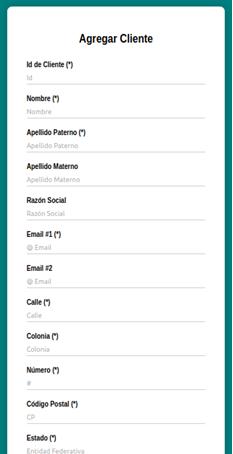
\includegraphics[scale=1]{fig5}
\end{minipage}
\end{figure}

\pagebreak

\begin{center}
VENTA
\end{center}
\begin{figure}[ht]
\begin{minipage}[t]{0.5\linewidth}
\caption {venta}
\centering
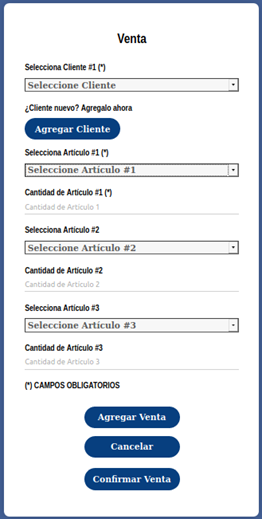
\includegraphics[scale=1]{fig6}
\end{minipage}
\begin{minipage}[t]{0.5\linewidth}
El siguiente módulo, posiblemente el más importante de todos, nos permite agregar ventas.\\

Dentro de este módulo debemos seleccionar el cliente al que se venderán los productos, en caso de que no lo tengamos registrado tenemos un botón en el que podemos agregar un nuevo cliente.\\

Después de seleccionar el cliente, debemos seleccionar los artículos para vender, en esta parte tenemos un menú desplegable que muestra todos los productos disponibles para vender y justo debajo debemos ingresar la cantidad a vender. \\

Tenemos la posibilidad de agregar 3 productos diferentes para cada venta. En este módulo hay más restricciones; Si desea vender una cantidad mayor que la que tenemos en stock, el sistema emite un mensaje de error y no se puede realizar la venta. Si se ingresa un valor incorrecto en la cantidad del producto, recibiremos un mensaje de error que indica que debemos ingresar los datos correctos.\\

Como tenemos todo el formulario completado correctamente, podemos seleccionar 3 opciones: Agregar venta, cancelar o confirmar la venta, para realizar la venta primero debemos seleccionar Agregar venta y se mostrará una vista de los productos que hemos agregado y qué es el precio que recibiremos por cada producto y el pago total por la venta.\\

Si desea cancelar la venta, seleccionaremos el botón Cancelar. \\
\end{minipage}
\end{figure}

\pagebreak

\begin{center}
PRODUCTO
\end{center}
\begin{figure}[ht]
\begin{minipage}[t]{0.5\linewidth}
\bigskip
\bigskip
\bigskip
\bigskip
El tercer módulo es "agregar producto", donde podemos agregar nuevos productos a nuestro inventario. En esta sección debemos ingresar el código de barras que pertenece al producto, la descripción del producto donde podemos poner el nombre del producto y algunas especificaciones adicionales que se necesitan, la marca del producto, el precio al que se compró proveedor, el precio al que se venderá al cliente, cuántas piezas agregamos al stock y seleccionamos el proveedor que nos vendió el producto, en caso de que un nuevo proveedor venda el producto, podemos seleccionar el botón "Agregar proveedor" para ingresar Los datos de un nuevo proveedor. \\

Una vez que hayamos completado correctamente el formulario, seleccionamos el botón "Registrar producto" donde se confirmará el registro. \\
\end{minipage}
\begin{minipage}[t]{0.5\linewidth}
\caption {Producto}
\centering
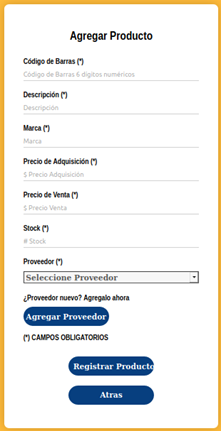
\includegraphics[scale=1]{fig7}
\end{minipage}
\end{figure}

\pagebreak

\begin{center}
CONSULTAR INVENTARIO
\end{center}

El siguiente módulo es "Consultar inventario", donde no hay muchas opciones aquí, ya que al ingresarlo solo se muestran los datos de los productos que tenemos en stock.\\

\begin{figure}[h]
\caption {Consultar inventario}
\centering
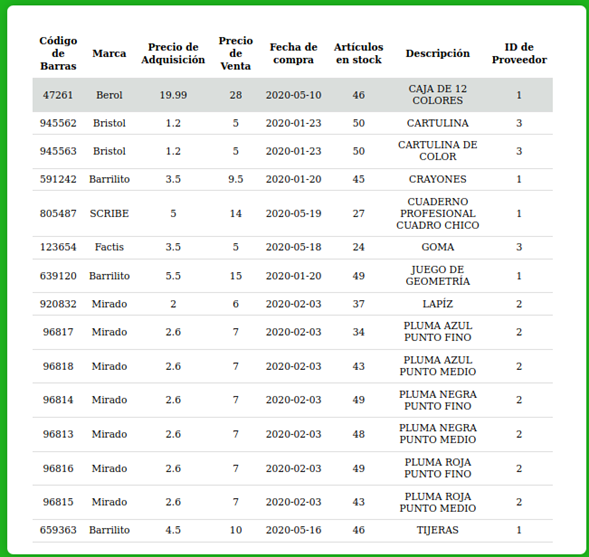
\includegraphics[width=\textwidth]{fig8}
\end{figure}

\pagebreak

\begin{center}
PROVEEDOR
\end{center}
\begin{figure}[ht]
\begin{minipage}[t]{0.5\linewidth}
\caption {Proveedor}
\centering
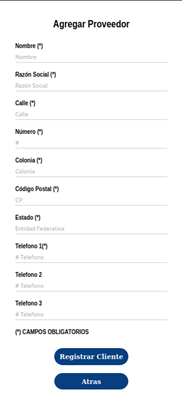
\includegraphics[scale=1]{fig9}
\end{minipage}
\begin{minipage}[t]{0.5\linewidth}
\bigskip
\bigskip
\bigskip
\bigskip
\bigskip
\bigskip
El quinto módulo nos permite agregar un nuevo proveedor, en este formulario debemos ingresar los datos correspondientes al nuevo proveedor; nombre, nombre comercial, dirección y 3 números de teléfono de contacto donde debemos ingresar al menos un número de teléfono. \\

Para registrar al proveedor, seleccione el botón para registrar al cliente y recibiremos un mensaje que ha registrado con éxito. 
\end{minipage}
\end{figure}

\pagebreak

\begin{center}
App
\end{center}
Como hoy en día todos usan sus teléfonos inteligentes para hacer todo, decidimos desarrollar también una aplicación. Esta aplicación funciona de la misma manera que la página web, con los mismos menús. \\

\begin{figure}[h]
\begin{minipage}[t]{0.5\linewidth}
\caption {Icono de la app}
\centering

\includegraphics[scale=0.16]{fig10}
\end{minipage}
\begin{minipage}[t]{0.5\linewidth}
\caption {Login de la app}
\centering
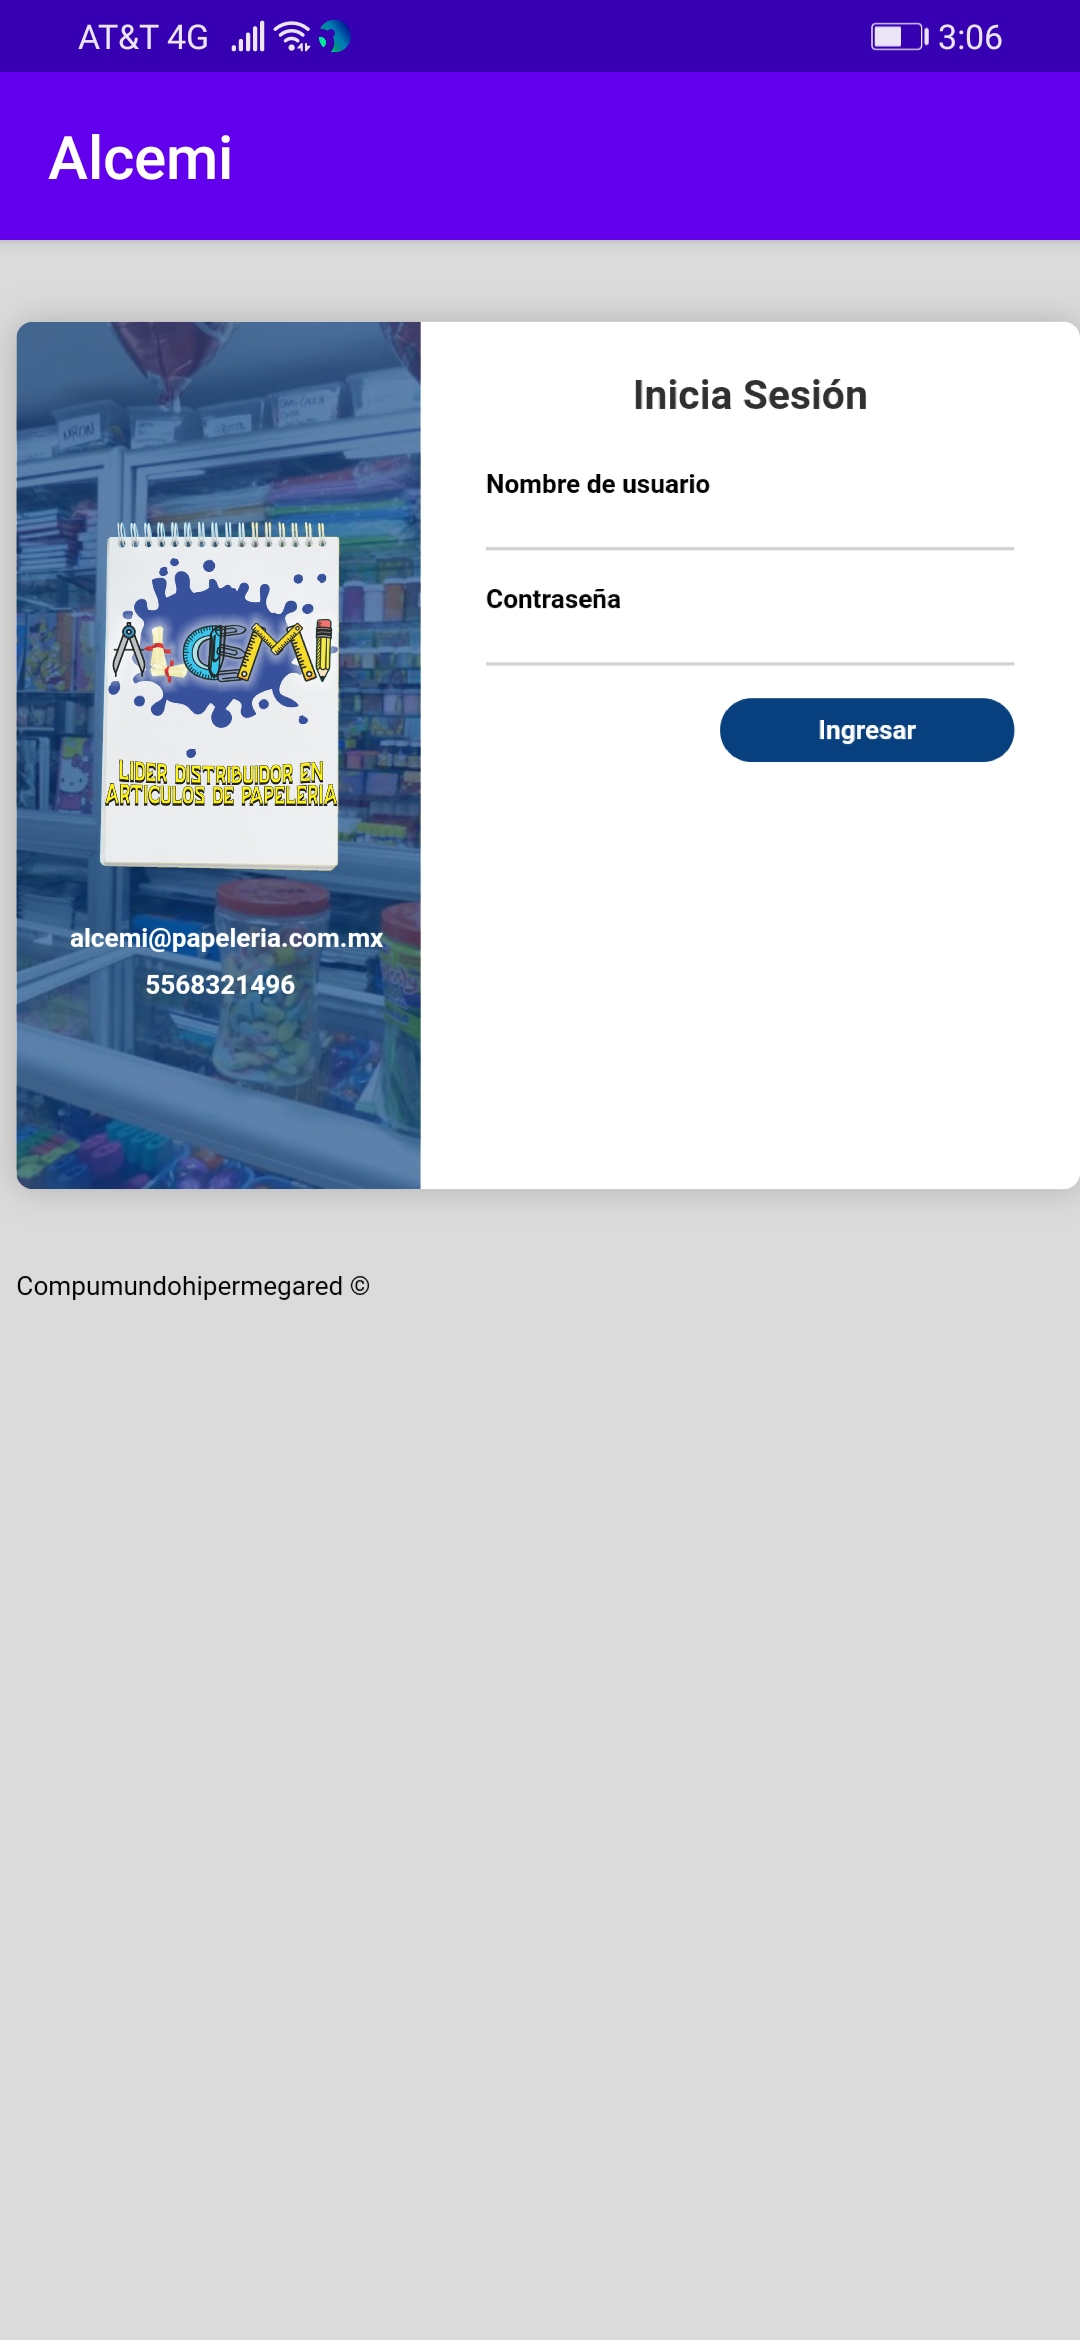
\includegraphics[scale=0.16]{fig11}
\end{minipage}
\end{figure}

\pagebreak

\begin{figure}[h]
\begin{minipage}[t]{0.5\linewidth}
\caption {Menu principal}
\centering
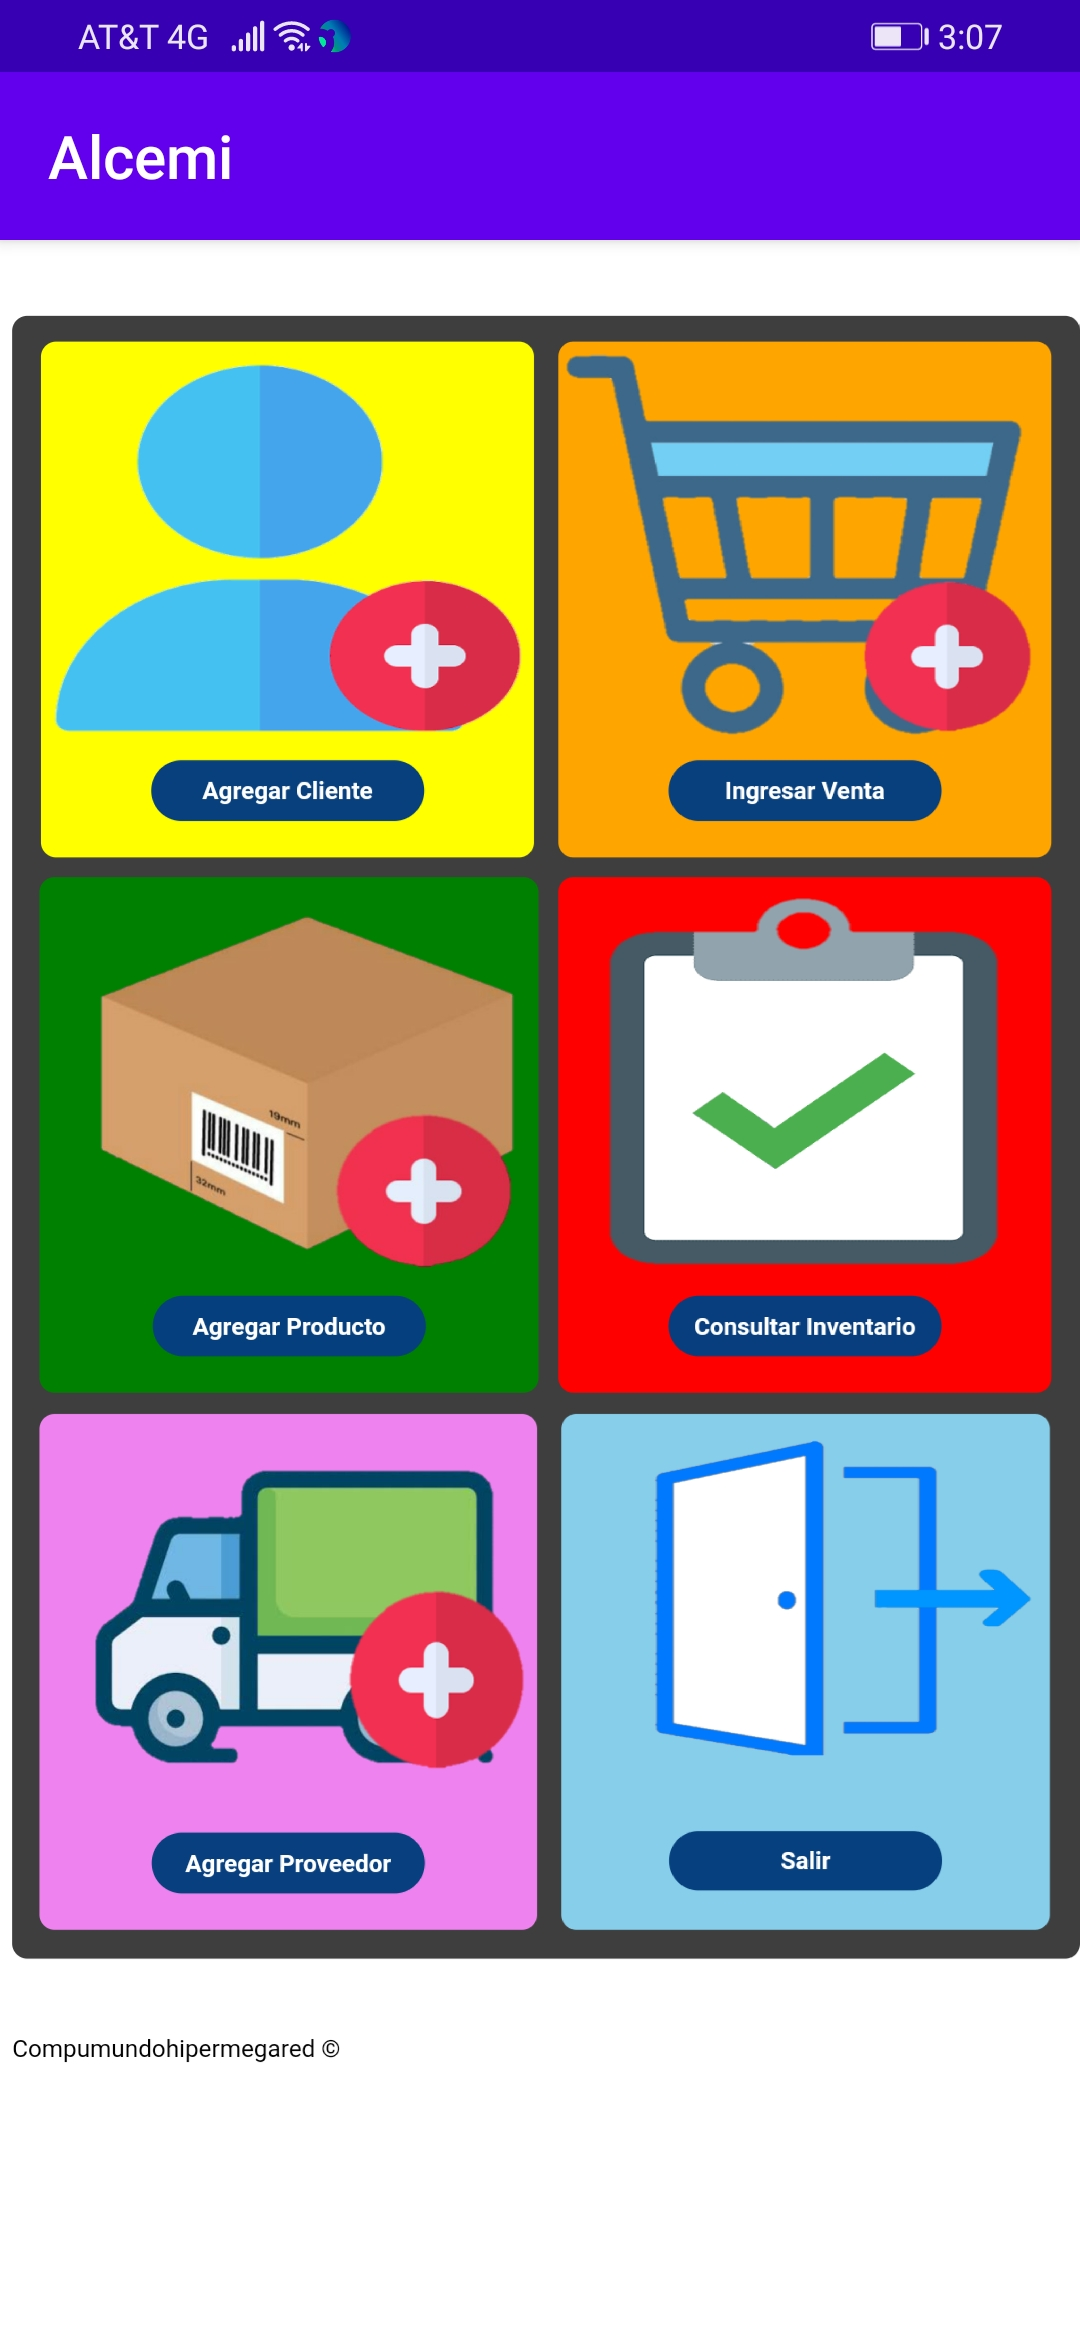
\includegraphics[scale=0.16]{fig12}
\end{minipage}
\begin{minipage}[t]{0.5\linewidth}
\caption {Haciendo una venta}
\centering
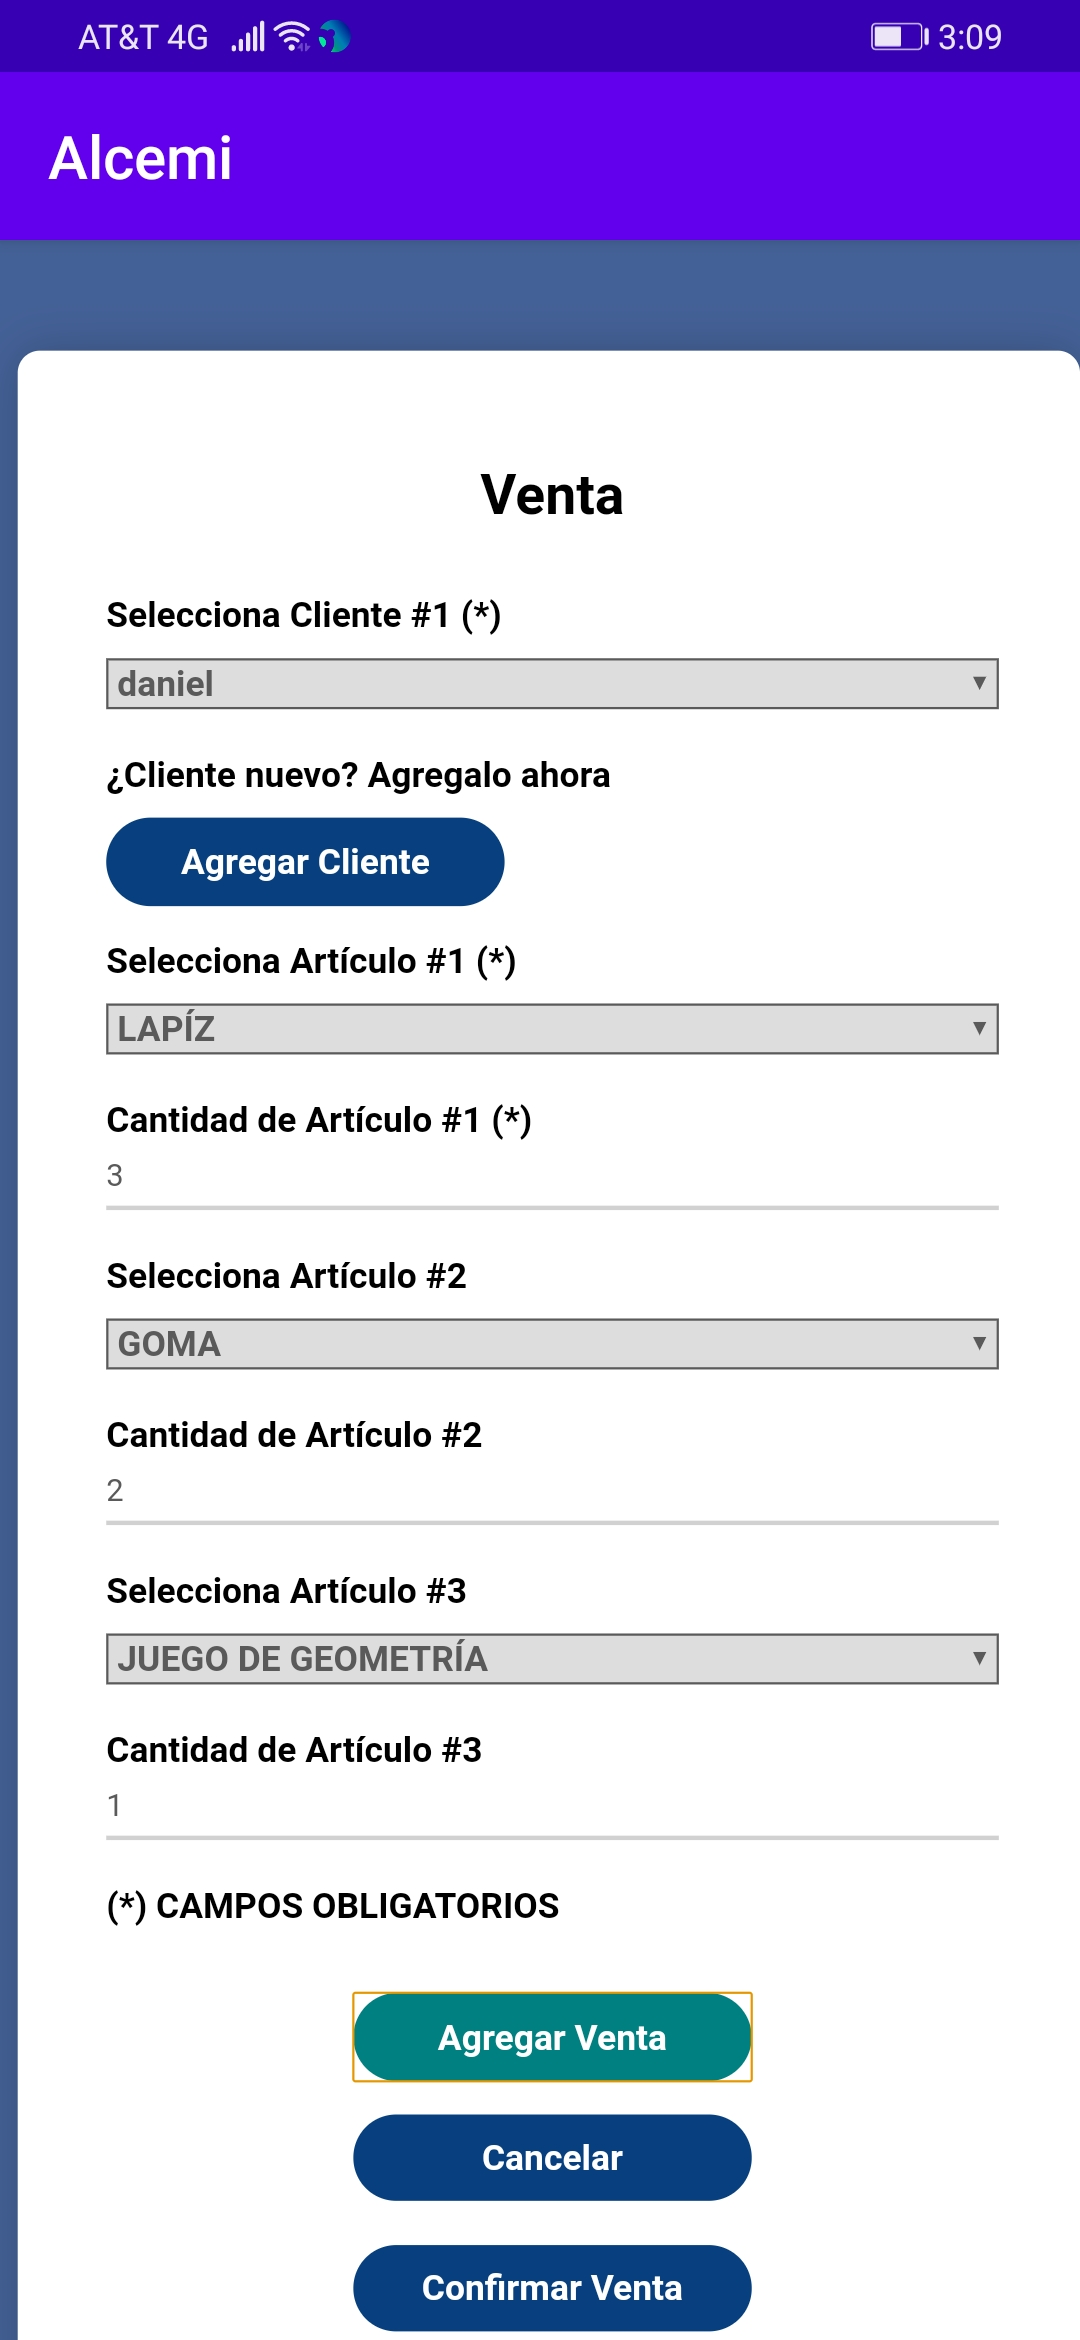
\includegraphics[scale=0.16]{fig13}
\end{minipage}
\end{figure}

\pagebreak

\begin{figure}[h]
\caption {Haciendo una venta}
\centering
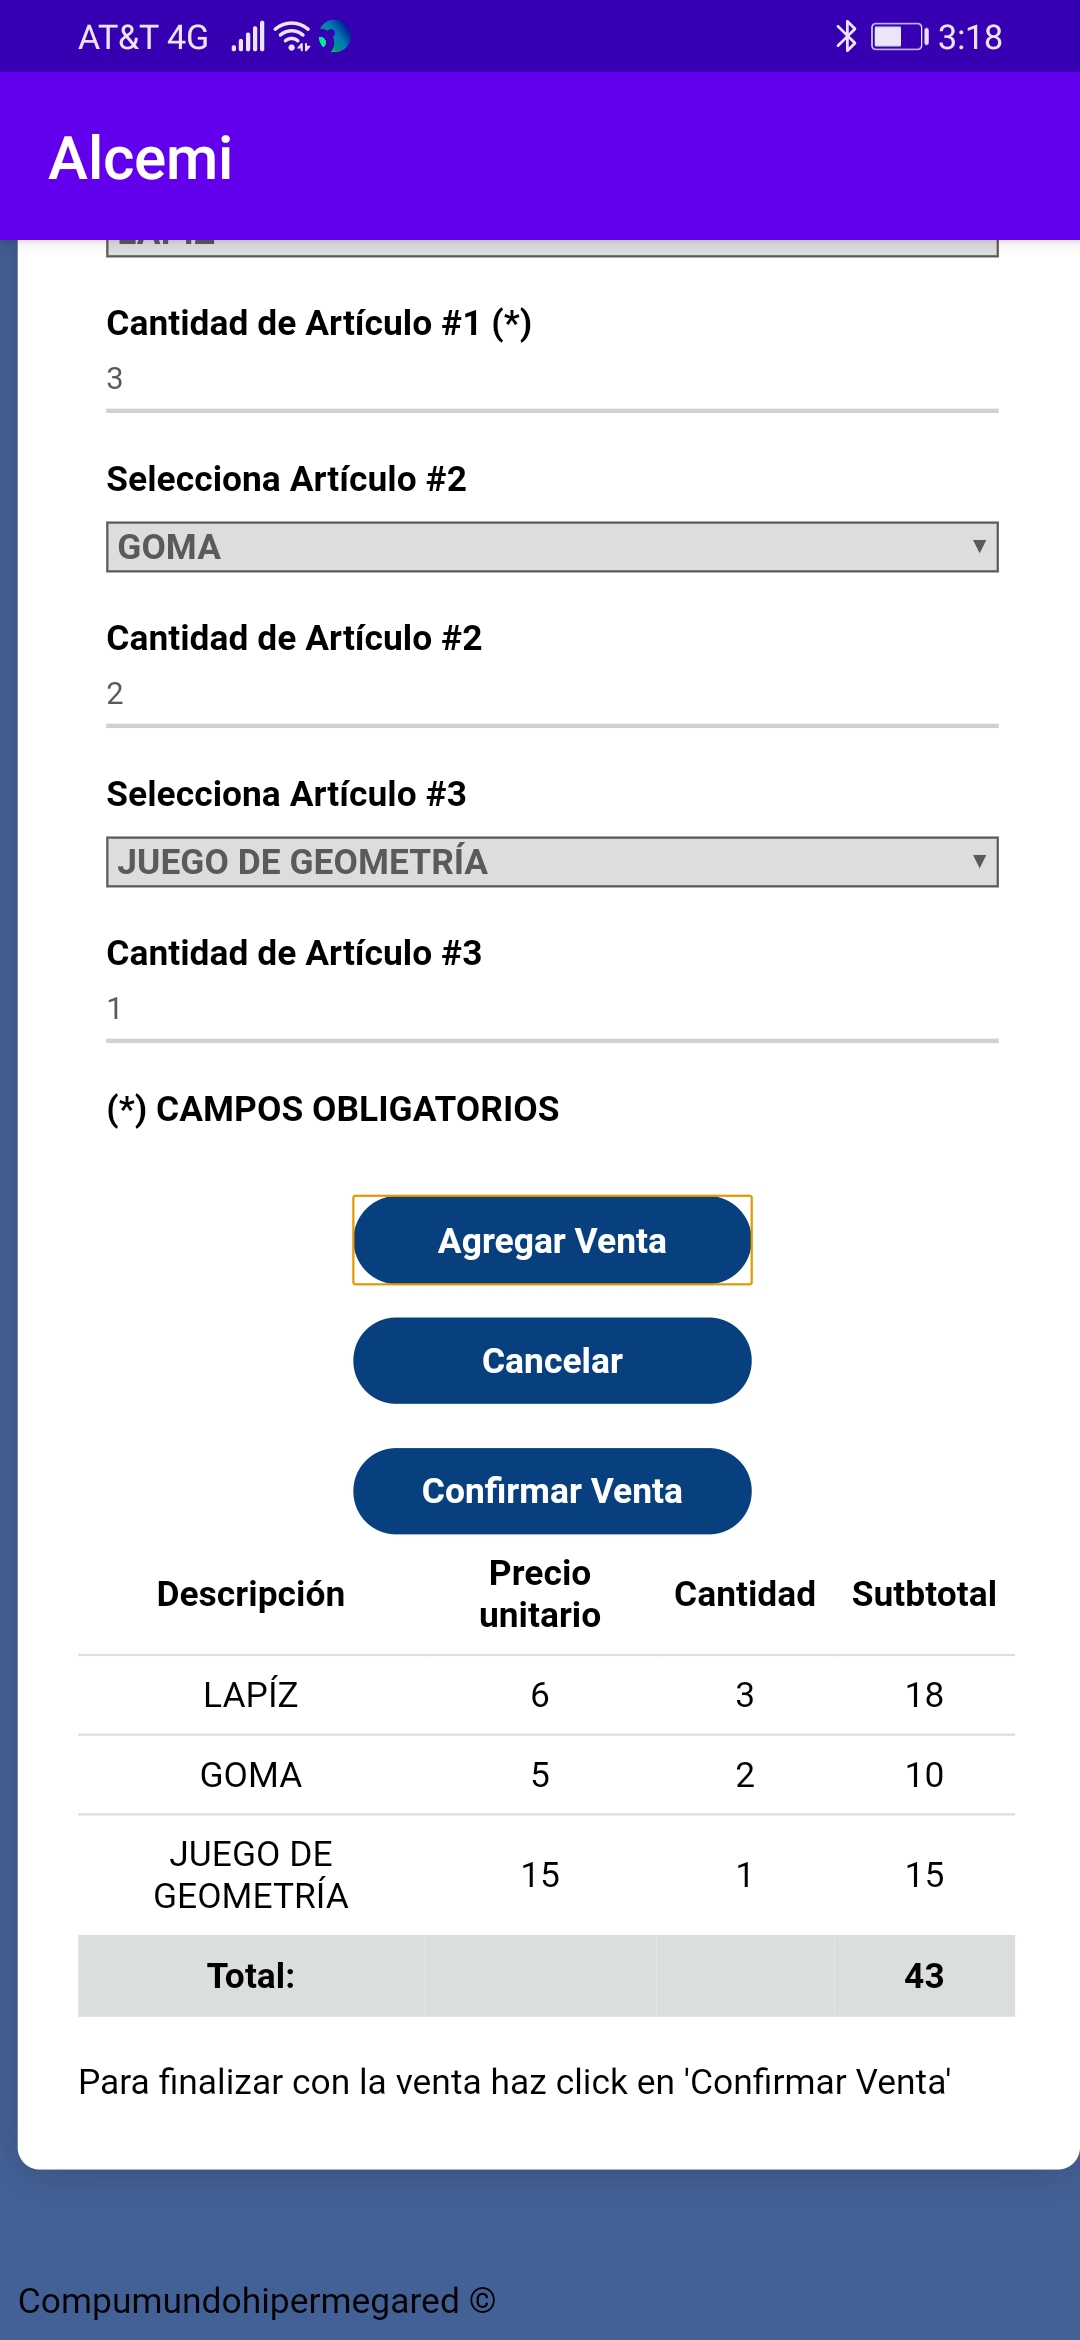
\includegraphics[scale=0.16]{fig14}
\end{figure}

\pagebreak

\section{Conclusiones}
César Gutierrez: Este proyecto fue muy util no solo para poner en practica todo lo aprendido en el curso sino tambien nos hizo aprender muchas cosas nuevas como lo relacionado directamente a la creacion de la app por ejemplo e inclusive en la creacion de este documento\\ 

Miguel Guzmán: La realización de este proyecto fue muy buena para el conocimiento adquirido, ya que no solo se utilizó lo que aprendimos en el curso, ya que a medida que avanzaba el proyecto surgieron más oportunidades para hacer cosas nuevas que nadie en el equipo había usado antes. Tales como la gestión y conexión entre los servidores. Al final del proyecto, nos damos cuenta de que no solo aprendimos bases de datos, sino también para crear un sistema posiblemente rentable y funcional.\\

Nava Escobar Jose Alfredo: Con base en lo realizado en este proyecto, puedo asegurar que el participar en él resultó muy enriquecedor, ya que pude poner en práctica los conocimientos adquiridos a lo largo del curso de teórico de bases de datos además de lo que como equipo aprendimos a lo largo del desarrollo de nuestro proyecto, el trabajo en equipo fue fundamental para la realización de este proyecto, creo que la colaboración fue la principal característica de este equipo de trabajo. Estoy satisfecho con el resultado final ya que pudimos crear y administrar una base de datos y de igual manera crear un sistema completo.\\

\end{document}















